% !TeX root=../main.tex
\chapter{تعاریف، اصول و مبانی نظری}
\label{def}
%\thispagestyle{empty} 
\section{مقدمه}
در مقالهٔ\cite{Nakamoto2009}، در کنار معرفی بیت‌کوین، روشی به نام 
%\RTLfootnote{\lr{Simplified Payment Verification (SPV)}}
\gls{Simplified Payment Verification (SPV)}
 (SPV) معرفی شده است. در این روش، امکانی به شبکه بیت‌کوین اضافه گشت که دسته‌ای از کاربران، بدون نیاز به راه‌اندازی یک گره کامل، بتوانند با اثبات مرکلی که از یک گره کامل دریافت می‌کنند، تایید کنند که یک تراکنش درون زنجیره بلوکی بیت‌کوین ثبت گردیده‌ است یا خیر. به این کاربران، کاربر سبک و به گره آن‌ها در شبکه بیت‌کوین، گره سبک گفته می‌شود. گره‌های سبک یا به عبارت دیگر گره‌هایی که در وضعیت تایید پرداخت ساده‌شده عمل می‌کنند، نیازی به ذخیرهٔ تمام زنجیره بلوکی وجود ندارند. این گره‌ها تنها سرایند زنجیره بلوکی را از شبکه دریافت و ذخیره می‌کنند.  هرچند که در این روش کاربران سبک نیاز به بارگیری تمام زنجیره بلوکی بیت‌‌کوین ندارند و تنها لازم است که سرایند بلوک‌ها را ذخیره کنند،‌ اما عملکرد صحیح آن‌ها در گرو ارتباط آن‌ها با یک گره کامل درست کار است. اگرچه گره‌های سبک می‌توانند تایید کنند که سرایند بلوک‌هایی که دریافت کرده‌اند اثبات کار صحیحی دارند یا خیر اما بدون داشتن تمام زنجیره بلوکی نمی‌توانند مطمئن شوند که تمام تراکنش‌های موجود در بلوک‌ها کاملا درست هستند.

آسیب‌پذیری دیگری که گره‌های سبک را تهدید می‌کند، عدم حفظ حریم خصوصی آن‌ها در مقابل گره‌های کاملی است که از آن‌ها درخواست اطلاعات می‌نمایند. یکی از اصلی‌ترین اطلاعاتی که گره‌های سبک از گره‌های کامل درخواست می‌کنند تراکنش‌های مربوط به آدرس(های) گره سبک است. کاربر سبک علاوه بر تراکنش مورد نظر، سرایند بلوکی که تراکنش در آن قرار دارد و همچنین اثبات مرکل وجود آن تراکنش در آن بلوک را دریافت می‌کند. در صورتی که گره سبک به صورت فاش اطلاعات آدرس خود را در اختیار گره کامل قرار دهد، گره کامل خواهد توانست اولا، ارتباط آدرس‌های بیت‌کوین گره سبک با آدرس آی‌پی وی را کشف نماید و در نهایت بفهمد که دارنده این آدرس در کدام موقعیت جغرافیایی قرار دارد. این امر می‌تواند باعث افشای هویت آن کاربر شود و حتی می‌تواند تهدیدی جانی برای کاربر سبک باشد اگر حملهٔ فیزیکی به آن فرد برای دزدیدن اطلاعات کیف پولش، که دارایی آن افشا شده است، صورت پذیرد. اگر کاربر سبک از 
%شبکه‌های حافظ گم‌نامی\RTLfootnote{\lr{Anonymity Network}}
\gls{Anonymity Network}
 مثل
%  تور\RTLfootnote{Tor} 
  \gls{Tor}
  استفاده نماید این امکان برای گره کامل وجود نخواهد داشت، هرچند که استفاده یا عدم استفاده از شبکه
 ثانیا، این امکان به گره کامل داده می‌شود که بتواند از این طریق ارتباط بین آدرس‌های یک شخص را در شبکه بیت‌کوین ساده‌تر کشف کند. کشف آن که کدام آدرس‌های بیت‌کوین مربوط به یک کاربر به خصوص است، می‌تواند به کشف الگوی رفتاری آن کاربر و در نتیجه کشف نسبی هویت آن منجر شود \cite{Ron2013}. از این رو فاش شدن هر دوی این اطلاعات حریم خصوصی کاربر سبک را نقض خواهد کرد.

به این ترتیب،‌ گره سبک به خاطر اعتماد به یک یا چند گره کامل و نقض حریم خصوصیش از امنیت کمتری نسبت به گره‌های کامل برخوردار است \cite{Sompolinsky2016}. از این رو تاکید می‌شود کاربرانی که مقدار زیادی بیت‌کوین را نگهداری یا مبادله می‌کنند، یا کاربرانی که می‌خواهند گم‌نامی آن‌ها حفظ شود از گره‌ کامل استفاده کنند. با این حال لازم است که تلاش شود امنیت، به ویژه گم‌نامی کاربران سبک تا حد امکان تامین گردد. چرا که فاش شدن اطلاعات بخشی از اعضای شبکه می‌تواند منجر به فاش شدن اطلاعات دیگر بخش‌های شبکه گردد.

در پروتکل فعلی بیت‌کوین برای حل مشکل فاش شدن آدرس مربوط به گره سبک نزد گره کامل متخاصم،  از فیلتر بلوم استفاده می‌شود \cite{Hearn2013}. در مقاله \cite{Gervais2014} توضیح داده ‌شد که استفاده از فیلتر بلوم از امنیت کافی برخوردار نیست. در این فصل پایان‌نامه به معرفی فیلتر بلوم، نحوهٔ استفاده آن در شبکه همتا‌به‌همتای بیت‌کوین و ضعف‌های آن به عنوان ابزاری جهت حفظ حریم خصوصی کاربران خواهیم پرداخت. در فصل بعد، مروری بر راه‌حل‌هایی که برای بهبود امنیت پروتکل فعلی ارائه شده است و همچنین روش‌هایی که جایگزین پروتکل فعلی هستند خواهیم کرد.


\section{بیت‌کوین}

رمزارز بیت‌کوین برای محقق ساختن اهدافی چون تبادل و نگه‌داری دارایی دیجیتال بدون نیاز به یک طرف سوم مورد اعتماد از یک الگورتیم 
\gls{Proof of Work} (\lr{PoW})
استفاده می‌کند\cite{Nakamoto2009}. الگوریتم اجماع اثبات کار بیت‌کوین تضمین می‌کند که بدون احتیاج به  وجود یک طرف قابل اعتماد در شبکه، کسی که توان پردازشی آن کمتر از $50$ درصد از شبکه باشد نتواند 
%حملهٔ دوبار خرج کردن\RTLfootnote{\lr{Double-Spend Attack}}
\gls{Double-Spend Attack}
را اجرا کند. تراکنش‌ها در بیت‌کوین درون بلوک‌هایی قرار می‌گیرند که این بلوک‌ها طبق الگوریتم اجماع کار تولید می‌شوند. هر بلوک به بلوک قبلی متصل است و تغییر در هر کدام از بلوک‌ها عملا ناشدنی است. در رمزارز بیت‌کوین، دارایی‌های هر کس در اکثر مواقع توسط کلید عمومی و خصوصی او مدیریت می‌شود. به این صورت که اگر یک فرد بخواهد مقداری بیت‌کوین دریافت کند، باید تراکنشی در زنجیرهٔ بلوکی بیت‌کوین قرار بگیرد که خروجی آن شرطی یا 
%نبشته\RTLfootnote{Script}
\gls{Script}
ای باشد که تنها آن فرد بتواند آن شرط را براورده کند. این شرط می‌تواند اشاره به کلید عمومی آن فرد باشد. مالک بیت‌کوین برای آن که این دارایی را به دیگری منتقل نماید، باید تراکنشی ایجاد کند که در ورودی آن ثابت کند که امکان براورده کردن این شرط را دارد. مثلا می‌تواند با کلید خصوصیش امضای دیجیتال انجام دهد و به این ترتیب ثابت کند که مالک آن کلید عمومی قرار گرفته در تراکنشی است که می‌خواهد آن را خرج نماید. به دلایلی چون خوانایی بهتر، کدگذاری‌های تشخیص خطا و غیره، معمولا به جای کلید عمومی از آدرس‌های بیت‌کوین استفاده می‌شود. این آدرس‌ها چکیدهٔ کلید عمومی هستند که توسط یک روش کدگذاری تشخیص خطا، کدگذاری شده‌اند.

به این ترتیب اگر مستقیما کلید عمومی فرد دریافت کننده در خروجی تراکنش قرار گیرد، به آن استاندارد
 \lr{P2PK}\LTRfootnote{\lr{Pay To Pubkey}}
 گفته می‌شود. و اگر خروجی آن، آدرس آن فرد باشد که با $1$ شروع شود به آن استاندارد 
  \lr{P2PKH}\LTRfootnote{\lr{Pay To Pubkey Hash}}
گفته می‌شود. این نوع نبشته بیشترین کاربرد را در بیت‌کوین دارد. جدیدا، با معرفی 
%سِگویت\RTLfootnote{Segwit} 
\gls{Segwit}
در بیت‌کوین، نبشته‌ای با نام 
  \lr{P2WPKH}\LTRfootnote{\lr{Pay to Witness Script Hash}}
معرفی شده است که با \lr{bc} شروع می‌شود. نوع نبشه‌ٔ دیگری برای شرایط خرج کردن وجود دارد به نام 
\lr{P2SH}\LTRfootnote{\lr{Pay To Script Hash}}
، در خروجی تراکنش، چکیدهٔ یک نبشته قرار می‌گیرد که خرج کننده باید خود آن نبشته‌ را ارائه نماید. نبشتهٔ شرط خروجی برای این دسته با $3$ شروع می‌شود.

بعضی از دادگان ذخیره‌شده در تراکنش‌ها و سرایند بلوک‌های بیت‌کوین به صورت 
اندین کوچک\LTRfootnote{Little-Endian}
ذخیره شده است، که از آن‌ها می‌توان به چکیده‌ها اشاره نمود. در شکل \ref{fig:endian} مقایسهٔ روش اندین کوچک و روش اندین بزرگ \LTRfootnote{Big-Endian} (روشی که انسان‌ها به صورت طبیعی اعداد را می‌نویسند) را برای دادهٔ \lr{\texttt{0x1A2B3C4D5E6F7080}} انجام داده است.

\begin{figure}[h]
	\centering
	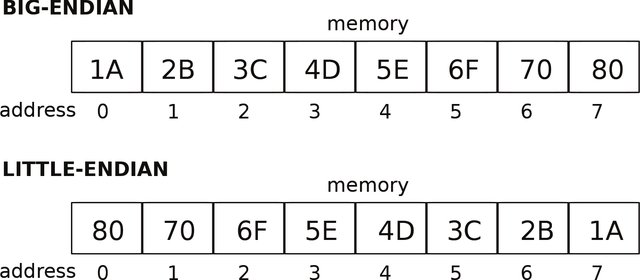
\includegraphics[width=0.7\linewidth]{image/endian}
	\caption{مقایسهٔ اندین کوچک و اندین بزرگ\cite{Grochowski2020}}
	\label{fig:endian}
\end{figure}


\subsection{گره‌ها‌}
گره‌‌های بیت‌کوین را می‌توان با توجه به کاری که انجام می‌دهند به انواع مختلفی دسته‌بندی کرد و طبق \cite{Antonopoulos2016} هر گره می‌تواند مجموعه‌ای از عملکرد‌های مسیریابی، پایگاه‌دادهٔ زنجیره‌ٔ بلوکی، استخراج و کیف پول باشد.
\paragraph{گره کامل}
در این پایان‌نامه منظور از گره کامل گره‌ای است که تمام زنجیرهٔ بلوکی را ذخیره کرده و قادر به مسیریابی و تبادل اطلاعات در شبکهٔ همتا‌به‌همتای بیت‌کوین باشد. گره کامل از بالاترین امنیت ممکن برخوردار بوده و قادر به اعتبارسنجی تمام تراکنش‌ها و بلوک‌ها، بدون افشای اطلاعاتش، است. پیاده‌سازی‌های مختلفی برای گره کامل بیت‌کوین وجود دارد که فرقی در عملکرد آن‌ها وجود ندارد. در این پایان‌نامه، گره کامل نرم‌افزار هستهٔ بیت‌کوین\cite{Bitcoincore.org} را اجرا می‌کند.

\paragraph{گره سبک}

پیاده‌سازی‌های نرم‌افزاری متعددی برای گره سبک یا به عبارت دیگر، کاربر SPV بیت‌کوین وجود دارد. مانند بیت‌کوین‌جی \cite{bitcoinj}، الکترام \LTRfootnote{\lr{Electrum}} 
\cite{Electrum}
و پیکوکوین\LTRfootnote{\lr{PicoCoin}}
\cite{Garzik}. 
اصطلاحا، به نرم‌افزار‌های گره سبک، کیف پول\LTRfootnote{\lr{Wallet}} نیز گفته می‌شود.

بیت‌کوین‌جی یک کتاب‌خانهٔ کاربر سبک (SPV) به زبان
% جاوا \RTLfootnote{\lr{Java}} 
 \gls{Java}
 است. این کیف پول مستقیما با استفاده از پروتکل‌های ارتباطی استاندارد تعریف شده در شبکهٔ همتا‌به‌همتای بیت‌کوین \cite{P2P_dev,P2P_ref} با گره کامل ارتباط برقرار می‌کند. بیت‌کوین‌جی از اکثر استاندارد‌های بیت‌کوین،‌از جمله فیلتر بلوم \cite{Hearn2013}  پشتیبانی می‌کند. در این پایان‌نامه به صورت کلی منظور از گره سبک یا کاربر \lr{SPV}، بیت‌کوین‌جی است. کاربر سبک بیت‌کوین‌جی به صورت همزمان می‌تواند به چند گره کامل متصل باشد و از طریق آن‌ها اطلاعاتش بروزرسانی گردد. کیف‌پول‌ 
بیت‌کوین ولت\LTRfootnote{\lr{Bitcoin Wallet}}، که برای سیستم‌عامل‌های اندروید و بلک‌بری توسعه پیدا کرده است، مثالی از کیف‌پول‌هایی است که از کتاب‌خانهٔ بیت‌کوین‌جی استفاده می‌کنند.

در پیاده‌سازی الکترام،‌ کاربر سبک مستقیما طبق پروتکل ارتباطی بیت‌کوین با گره کامل مبادلهٔ اطلاعات نمی‌کند. گره کاملی که زنجیره بلوکی بیت‌کوین را ذخیره کرده‌است،‌ لازم است برای ارائه خدمات به کاربران سبکی که از الکترام استفاده می‌کنند،‌ سرور 
الکترام‌ایکس\LTRfootnote{\lr{ElectrumX}}
\cite{ElectrumX}
را در کنار نرم‌افزار گره کامل (هسته‌ٔ بیت‌کون) راه‌اندازی نماید. در این پیاده‌سازی، برخلاف بیت‌کوین‌جی، گره سبک هم‌زمان به چند سرور الکترام‌ایکس متصل نمی‌شود. بلکه به صورت تصادفی یک سرور را انتخاب می‌کند و به آن متصل می‌گردد. کاربر سبک خودش می‌تواند تعیین کند که به چه سروری متصل گردد. از این رو کاربر سبک می‌تواند اطلاعاتش را تنها از گره کاملی که به آن اعتماد دارد به روز رسانی نماید.  همچنین در پروتکل ارتباطی گره سبک الکترام با سرور الکترام‌ایکس از فیلتر بلوم استفاده نمی‌شود. این ویژگی‌ها امنیت این پیاده‌سازی را با ابهام مواجه کرده است \cite{Alison2014}. 

پیکوکوین،‌ یک کتاب‌خانه بیت‌کوین به زبان سی\LTRfootnote{\lr{C}} است. این کتاب‌خانه امکان استفاده به عنوان یک کیف‌پول بیت‌کوین و یک گره کامل را فراهم می‌کند. علاوه بر این، امکان ساخت نرم‌افزارهایی که مرتبط با بیت‌کوین هستند را ممکن می‌کند. این کیف پول از استاندارد ارتباطی بیت‌کوین تبعیت کرده و از فیلتر بلوم استفاده می‌کند، همچنین می‌تواند مستقیما به گره‌های کامل بیت‌کوین، بدون نیاز به راه‌اندازی سروری مجزا در سمت گره کامل، متصل شود.

در این پژوهش هرگاه از گره سبک یا کاربر SPV صحبت می‌شود منظور کیف‌پول بیت‌کوین‌جی \cite{bitcoinj} و هر گاه از گره کامل صحبت می‌شود منظور نرم‌افزار
%هستهٔ بیت‌کوین\RTLfootnote{Bitcoin-core} 
\gls{Bitcoin-core}
\cite{Bitcoincore.org}
است.


\subsection{شبکه همتا‌به‌همتای بیت‌کوین}
\label{P2PNetwork}

گره‌های شبکهٔ بیت‌کوین بر اساس یک پروتکل استاندارد با یکدیگر به تبادل پیام می‌پردازند. گره‌های کامل در شبکه بیت‌کوین بعد از آن‌که بلوک‌ها و تراکنش‌های جدید را تصدیق کردند، آن‌ها را به دیگر گره‌ها ارسال می‌کنند. علاوه بر این، گره‌های سبک می‌توانند از پروتکل ارتباطی بیت‌کوین جهت ارتباط با گره‌های کامل استفاده کنند.

تمام  ارتباطات همتا‌به‌همتا در بیت‌کوین در بستر TCP برقرار می‌شوند و تمام پیام‌ها از قالب یکسانی پیروی می‌کنند. رشتهٔ آغازین پیام‌ها و مقدار پیش‌فرض شمارهٔ درگاه با توجه به اینکه پیام در شبکهٔ اصلی، تست یا در حالت تست رگرسیون استفاده می‌شود تفاوت می‌کند. جدول \ref{table:PortandString} این مقادیر را نشان می‌دهد. یک گره می‌تواند از شمارهٔ درگاهی متفاوت در یک شبکه استفاده نماید.



\begin{xltabular}{\textwidth}{|c|c|c|X|}
	\caption{شبکه‌های مختلف بیت‌کوین\label{table:PortandString}}\\
	\hline
	\textbf{شبکه} & \textbf{درگاه پیش‌فرض} & \textbf{رشته‌ٔ آغازین} & \textbf{توضیحات} \\
	\hline \hline 
	اصلی & 8333 & \lr{\texttt{0xf9beb4d9}} & {%
		شبکهٔ اصلی بیت‌کوین.
	}\\
	\lr{Mainnet} & & & {%
		در این شبکه بیت‌کوین دارای ارزش واقعی است.
	} \\
	\hline
	تست & 18333 & \lr{\texttt{0x0b110907}} & {%
		شبکهٔ آزمایشی بیت‌کوین
	}\\
	\lr{Testnet} & & & {%
		برای توسعه دهندگان بهتر و کم هزینه‌ تر است که از شبکهٔ آزمایشی بیت‌کوین استفاده کنند. چرا که بیت‌کوین‌ در آن دارای ارزش واقعی نیست.
	} \\
	\hline
	تست رگرسیون & 18444 & \lr{\texttt{0xfabfb5da}} & {%
		حالت تست رگرسیون
	}\\
	\lr{Regtest} & & & {%
		گاهی در توسعه یک کاربرد نیازی نیست که با گره‌های تصادفی در ارتباط باشیم یا بلوک‌های تصادفی تولید شده را بررسی کنیم. در این شرایط از حالت تست رگرسیون بیت‌کوین استفاده می‌کنیم. در این حالت می‌توان محیط را کنترل کرد و تعیین کرد که چه زمانی یک بلوک جدید ساخته شود.
	} \\
	\hline
	
	
\end{xltabular}


علاوه بر این تمام پیام‌های شبکه‌ٔ همتا‌به‌همتای بیت‌کوین شامل سرایندی یکسان هستند که قالب این سرایند مطابق جدول \ref{table:p2pheader} است.

\begin{xltabular}{\textwidth}{|c|X|}
	\caption{قالب سرایند تمام‌ پیام‌ها در شبکهٔ همتا‌به‌همتای بیت‌کوین \label{table:p2pheader}}\\ \hline
	\textbf{نام} & {\textbf{توضیحات} } \\
	\hline \hline
	\lr{start string}&{%
		بایت‌هایی که در جدول \ref{table:PortandString} توضیح داده شد که نشان دهندهٔ شبکه‌ای است که این پیام در آن تولید شده است.
	}\\
	\hline
	
	\lr{command name} & {%
		رشته‌ای در استاندارد 
%		اَسکی
		\gls{ASCII}\LTRfootnote{ASCII}
		است که مشخص می‌کند چه نوع پیامی در 		
		\gls{Payload}\LTRfootnote{Payload}
		قرار گرفته است. اندازهٔ این قسمت ۱۲ کاراکتر است و بایت‌های بعد از نام پیام برابر صفر (\texttt{0x00}) خواهند بود. به عنوان مثال برای پیام \texttt{Version} خواهیم داشت:
		\lr{\texttt{version\textbackslash0\textbackslash0\textbackslash0\textbackslash0\textbackslash0}}.
	}\\
	\hline
	
	\lr{payload size} & {%
		اندازه بایت‌های پیام داخل پایه‌بار را مشخص می‌کند. حداکثر تعداد بایت‌ مجاز در پایه‌بار ۳۲ مگابایت‌ (\lr{‍‍``MAX\_SIZE''}) است. پیام‌های بزرگ‌تر از این مقدار دورانداخته می‌شوند. پیام‌هایی مانند \texttt{VerAck}   بدون پایه‌بار هستند.
	}\\
	\hline
	
	\lr{checksum} & {%
		چهار بایت اول حاصل 
		\lr{SHA256(SHA256(payload))}
		است. اگر پایه‌بار خالی باشد، مانند پیام‌های \texttt{VerAck} و \texttt{GetAddr}، مقدار این بخش برابر 
		\lr{\texttt{0x5df6e0e2}}
		بوده که معادل 
		\lr{SHA256(SHA256(
			\rl{رشتهٔ خالی}
			))}
		است.
	}\\
	\hline
	
\end{xltabular}  

\subsubsection{یافتن همتا}

اولین گامی که هر گره در شبکهٔ همتا‌به‌همتای بیت‌کوین انجام می‌دهد، یافتن گره‌های (همتا‌های) دیگر و اتصال به آن‌ها است. از آن‌جایی که یک گره در زمان راه اندازی، آدرس آی‌پی گره‌های کامل فعال را ندارد، از یک یا چند سرور 
\LTRfootnote{\lr{Domain Name System}}\lr{DNS} 
که آدرس‌ آن‌ها در کد بیت‌کوین‌جی از پیش قرارگرفته است پرسمان انجام می‌دهد. پاسخ دریافت شده شامل آدرس یک یا چند گره کامل است که ارتباطات ورودی را قبول می‌کنند. علاوه بر این تعدادی آدرس گره کامل در هر ورژن از کدهای بیت‌کوین‌جی قرار دارد که در زمانی که آن ورژن مشخص منتشر می‌شده فعال بوده‌اند. 
\subsubsection{اتصال به همتا}
بعد از آن‌که کاربر جدید آدرس آی‌پی یک یا چند گره کامل را بدست آورد، برای آن گره‌(ها) پیام \texttt{version} را ارسال می‌کند. این پیام برای ایجاد ارتباط ارسال می‌شود و شامل اطلاعاتی از گره ارسال کننده است. این اطلاعات در جدول \ref{table:VersionMessage} توضیح داده شده است. گره دریافت کننده نیز یک پیام \texttt{version} را که شامل اطلاعات خودش است، ارسال می‌کند. هر دو گره به محض دریافت پیام \texttt{version} پیام \texttt{verack} را برای گره مقابل ارسال می‌نماید. پیام \texttt{verack} بدون
%پایه‌بار\RTLfootnote{Payload}
\gls{Payload}
است و به گره دریافت کننده اطلاع می‌دهد که آماده دریافت پیام‌‌های بعدی است.


\begin{xltabular}{\textwidth}{|c|X|}
	\caption{
		قسمت‌های پیام \texttt{version} در شبکه همتا‌به‌همتای بیت‌کوین
		\label{table:VersionMessage}}\\
	\hline
	\textbf{نام} & {\centering
		\textbf{توضیحات}		
	} \\
	\hline
	\hline
	\lr{version} & {
		بالاترین نسخهٔ پروتکلی که توسط گره ارسال کننده شناخته می‌شود.	در زمان نگارش این پایان‌نامه، بالاترین نسخه پروتکل بیت‌کوین 70015 است که در سال ۲۰۱۷ منتشر شده است.
	} \\
	\hline
	\lr{services} & {
		خدماتی که گره ارسال‌کننده پشتیبانی می‌کند را مشخص می‌کند. برای گره‌های سبکی مثل بیت‌کوین‌جی، مقدار آن برابر \texttt{0x00} است.
	} \\
	\hline
	\lr{timestamp} & {
%		ساعت یونیکس\RTLfootnote{\lr{Unix time}} 
		\gls{Unix time}\LTRfootnote{\lr{Unix time}}
		با توجه به ساعت گره ارسال کننده در زمان ارسال پیام.
	} \\
	\hline
	\lr{addr\_recv services} & {
		سرویس‌هایی که از دید گره ارسال‌کننده، توسط گره گیرنده پشتیبانی می‌شود. فرمت نمایش آن مانند قسمت services است. اگر گره ارسال‌کننده، بیت‌کوین‌جی باشد، همیشه به صورت پیش‌فرض مقدار این قسمت را برابر \texttt{0x00} قرار می‌دهد.
	} \\
	\hline
	\lr{addr\_recv port} & {
		شماره پورت گره گیرنده از دید گره ارسال‌کننده.
	}\\
	\hline
	\lr{addr\_trans services} & {
		خدماتی که گره ارسال‌کننده پشتیبانی می‌کند را مشخص می‌کند. یکسان با قسمت services باید باشد.
	}\\
	
	\hline
	\lr{addr\_trans IP address} & {
		آدرس آی‌پی گره ارسال کننده.
	}\\
	
	\hline
	\lr{addr\_trans port} & {
		شماره پورت گره ارسال کننده.
	}\\
	
	\hline
	\lr{nonce} & {
		تک‌شمار، یک عدد تصادفی است که اگر یک گره،‌ یک پیام با تک‌شماری مشابه با تک‌شمار ارسالی دریافت کرد، ارتباط را قطع نماید. (قسمت تک‌شمار در نسخهٔ \lr{$0.1.6$} بیت‌کوین اضافه شده و هدفش آن است که گره متوجه شود که به خودش متصل نشده باشد)
		\LTRfootnote{  \lr{\url{https://github.com/bitcoin/bitcoin/commit/cc0b4c3b62367a2aebe5fc1f4d0ed4b97e9c2ac9}}}.
	}\\
	\hline
	\lr{user\_agent bytes} & {
		تعداد بایت‌هایی که پیام قسمت \lr{user\_agent} (قسمت بعدی) استفاده کرده است.
	}\\
	
	\hline
	\lr{user\_agent} & {
		نوع برنامه کاربر را معین می‌کند. مثلا:
	}\\
	
	&  {%
		۱. بیت‌کوین‌جی: 
		\lr{/bitcoinj:1.0/MultiBit:1.0(Windows)/}} \\
	&  {%
		۲. هستهٔ بیت‌کوین (گره کامل): 
		\lr{/Satoshi:0.20.0/(70015)/}} \\
	
	\hline
	\lr{start\_height} & {
		ارتفاع بهترین زنجیره‌ بلوکی گره ارسال کننده در این قسمت قرار گرفته می‌شود. در صورتی که کاربر SPV باشد، ارتفاع بهترین زنجیره سرایند بلوک‌‌ها قرار داده می‌شود.
	}\\
	
	\hline
	\lr{relay} & {
		قرار دادن این بخش در پیام اختیاری است. این بخش در \cite{Hearn2013} به همراه پیشنهاد استفاده از فیلتر بلوم در بیت‌کوین معرفی شده است. مقدار آن صحیح (\texttt{0x01}) یا غلط (\texttt{0x00}) است. در صورتی که صحیح باشد، یا از آن استفاده نشود، تغییری در پروتکل ایجاد نمی‌شود. ولی در صورتی که غلط باشد، قبل از آن‌که کاربر ارسال کننده، پیام‌های \texttt{filterload} و \texttt{filterclear} را ارسال کرده باشد، هیچ پیام \texttt{inv} یا \texttt{tx} به آن ارسال نمی‌شود. این کار باعث می‌شود که در فاصلهٔ زمانی انجام 
%		دستداد \RTLfootnote{Handshake}
		\gls{Handshake}\LTRfootnote{Handshake}
		(ارسال پیام \texttt{version}) و فرستادن فیلتر بلوم، کاربر سبک تحت سیل پیام‌های گره‌کامل قرار نگیرد. 
	}\\
	
	
	\hline
\end{xltabular}

زمانی که اتصال با یک گره کامل برقرار شد، پیام \texttt{getaddr} برای گره کامل فرستاده می‌شود تا آدرس آی‌پی گره‌های کامل فعالی که گره دریافت‌کننده به آن‌ها متصل است در قالب پیام \texttt{addr} برای گره فرستنده ارسال شود. گره فرستنده همتا‌های فعال خودش را نیز در قالب پیام \texttt{addr} برای گره کامل گیرنده ارسال می‌کند.

\subsubsection{هم‌گام سازی گره سبک}
از این قسمت به بعد تنها به بررسی فعالیت‌های گره سبک در شبکه می‌پردازیم و هم‌گام‌سازی دیگر گره‌های شبکه مورد بررسی قرار نمی‌گیرند. کاربر سبک بعد از اتصال اولیه به یک گره کامل، نیاز دارد که سرایند بلوک‌های زنجیرهٔ بلوکی را دریافت نماید به این کار 
%هم‌گام‌سازی \RTLfootnote{Synchronization}
 \gls{Synchronization}
 گفته می‌شود. همان‌طور که گفته شد کاربر سبک به جای ذخیره‌سازی و تصدیق تمام زنجیرهٔ بلوکی،‌ تنها سرایند آن را ذخیره می‌کند. حجم سرایند یک بلوک $80$ بایت است. در گره‌های کامل، که می‌خواهند تمام زنجیره بلوکی را دریافت نمایند، این فرایند به دو صورت
%«ابتدا-بلوک\RTLfootnote{Blocks-First}»
«\gls{Blocks-First}»
یا
«\gls{Headers-First}»
قابل انجام است که در این‌جا به توضیح آن‌ها پرداخته نمی‌شود. گره سبک در گام اول هم‌گام‌سازی لازم است که 
%بهترین سراید زنجیرهٔ بلوکی \RTLfootnote{\lr{Best header chain}} 
\gls{Best header chain}
را دانلود کند. سرایند زنجیرهٔ بلوکی، زنجیره‌ای از سرایند بلوک‌ها است که هر کدام از سرایند‌ها به سرایند بلوک قبل خود اشاره می‌کند. بهترین سرایند زنجیرهٔ بلوکی، زنجیره‌ای است که دشوارترین بازآفرینی را داشته باشد. 

گره سبک برای دریافت سرایند زنجیرهٔ بلوکی، پیام \texttt{getheaders} را برای گره کاملی (گره هم‌گام‌ساز) که می‌خواهد با آن همگام شود ارسال می‌کند. جدول \ref{table:GetHeadersMessage} بخش‌های مختلف این پیام را توضیح می‌دهد و شکل \ref{fig:getheaders} مثالی از یک پیام \texttt{getheaders} است که گره سبک برای اولین‌بار برای گره هم‌گام‌ساز ارسال می‌کند.



\begin{xltabular}{\textwidth}{|c|X|}
	\caption{
		قسمت‌های پیام \texttt{getheaders} در شبکه همتا‌به‌همتای بیت‌کوین
		\label{table:GetHeadersMessage}}\\
	\hline
	\textbf{نام} & {\textbf{توضیحات}} \\
	\hline \hline
	\lr{version} & {%
		شماره‌ٔ نسخه‌ٔ پروتکل. شبیه آنچه در پیام \texttt{version} ارسال شد.
	} \\
	
	\hline
	
	\lr{hash count} & {%
		تعداد چکیده‌هایی که در بخش بعدی پیام قرار می‌گیرند، در این قسمت تعیین می‌شوند. محدودیتی در تعداد چکیده‌های ارسالی نیست. اما اندازه کل پیام باید کمتر از \lr{‍‍``MAX\_SIZE''} (۳۲ مگابایت) باشد.
	} \\
	\hline
	
	
	\lr{block header hashes} & {%
		چکیدهٔ یک یا چند سرایند بلوکی که گره ارسال کننده آن‌ها را در حافظهٔ خود دارد. ترتیب چکیده‌ها از بالاترین ارتفاع بلوک (جدید‌ترین) به پایین‌ترین ارتفاع است. به این ترتیب به گره دریافت‌کننده‌ٔ پیام این امکان داده می‌شود که جدیدترین چکیدهٔ سرایندی که با هم مشترک هستند را پیدا کند. اگر گره سبکش تازه راه‌اندازی شده‌ باشد در این قسمت، چکیدهٔ بلوک جنسیس (\lr{6fe2…0000}) را که در نرم‌افزارش از ابتدا وجود داشته است، قرار می‌دهد.
	} \\
	\hline
	
	\lr{stop hash} & {%
		این قسمت چکیدهٔ آخرین بلوکی است که گره ارسال‌کننده می‌خواهد دریافت کند. با صفر قراردادن آن، طولانی‌ترین پاسخ ممکن از گره کامل تقاضا می‌شود. حداکثر تعداد سرایندی که گره کامل دریافت کنندهٔ این پیام پاسخ می‌دهد، $2000$ سرایند است. برای دریافت بیشتر از این مقدار، این پیام در چند نوبت ارسال می‌شود
	}\\
	\hline
	
\end{xltabular}

\begin{figure}[h]
	\centering
	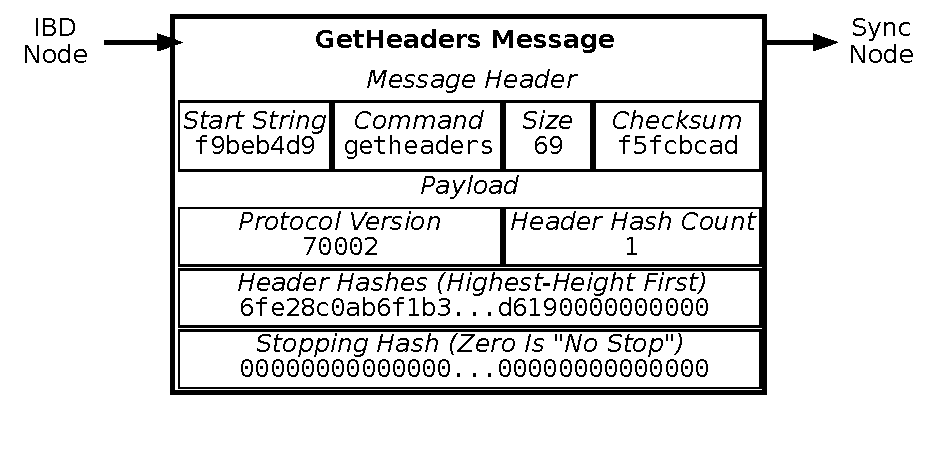
\includegraphics[width=0.7\linewidth]{image/getheaders}
	\caption{مثالی از پیام \texttt{getheaders} در همگام‌سازی اولیهٔ یک گره جدید}
	\label{fig:getheaders}
\end{figure}


گره هم‌گام‌ساز در پاسخ به پیام \texttt{getheaders} در شکل \ref{fig:getheaders} دنبال بلوکی با چکیده مشخص شده می‌گردد و می‌یابد که این بلوک برابر بلوک شمارهٔ صفر (بلوک جنسیس) است. به این ترتیب $۲۰۰۰$ سرایند بلوک را که از بلوک شمارهٔ یک آغاز می‌شوند در قالب پیام \texttt{headers} برای گره درخواست دهنده ارسال می‌کند. قالب این پیام در جدول \ref{table:HeadersMessage} مشخص شده‌ است. شکل \ref{fig:headers} مثالی از پیام بازگردانده شده توسط گره هم‌گام‌ساز است.

\begin{table}[!h]
	\centering
	\caption{
		قسمت‌های پیام \texttt{headers} در شبکه همتا‌به‌همتای بیت‌کوین
		\label{table:HeadersMessage}}
	\begin{tabular}{|c|r|}
		\hline
		\textbf{نام} & {\textbf{توضیحات}} \\
		\hline \hline
		
		\lr{count} & {%
			تعداد سرایند‌های بلوک قرار گرفته در بخش بعدی این پیام. (حداکثر $2000$)
		} \\
		\hline
		
		\lr{headers} & {%
			سرایند‌ بلوک‌ها در این قسمت قرار می‌گیرند.
		} \\
		\hline
	\end{tabular}
\end{table}

\begin{figure}[!h]
	\centering
	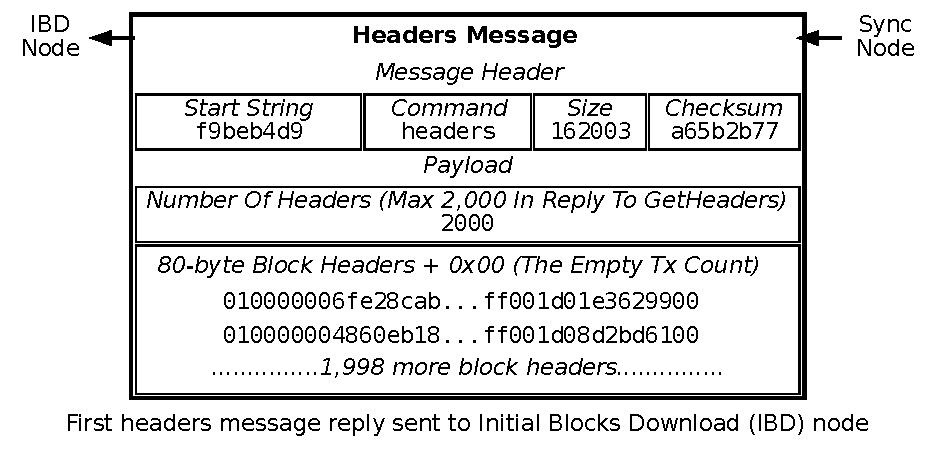
\includegraphics[width=0.7\linewidth]{image/headers}
	\caption{مثالی از پیام \texttt{headers} در همگام‌سازی اولیهٔ یک گره جدید}
	\label{fig:headers}
\end{figure}

وقتی گره سبک پاسخ شکل \ref{fig:headers} را دریافت کرد، فورا صحت آن را بررسی کرده و مجددا پیام  \texttt{getheaders} جدیدی برای گره همگام‌ساز برای گرفته باقیمانده سرایند‌ها ارسال می‌کند. این فرایند تا گرفتن کامل سرایند‌ها ادامه پیدا می‌کند. در زمان نوشتن این پایان‌نامه، حجم تمام سرایند‌های زنجیرهٔ بلوکی ۵۰ مگابایت است. پس از اتمام دانلود سرایند‌های زنجیرهٔ  بلوکی، گره سبک آخرین پیام \texttt{getheaders} را برای چند همتای دیگر ارسال کرده و پاسخ آن‌ها را با پاسخ گره هم‌گام‌ساز ابتدایی مقایسه می‌کند. به این ترتیب مطمئن می‌شود که بهترین سرایند زنجیرهٔ بلوکی را دریافت کرده است. 

\subsubsection{انتشار}

زمانی که گره کامل یک بلوک جدید را دریافت می‌کند، پیام \texttt{inv} را برای همهٔ همتا‌هایش (چه گره کامل چه گره سبک) ارسال می‌کند. پیام ارسال شده دارای یک 
%مدخل فهرست \RTLfootnote{Inventory} 
\gls{Inventory}
مربوط به بلوک جدید است. یک مدخل فهرست، شامل یک علامت نوع داده و یک  چکیده داده به عنوان مشخص‌کنندهٔ آن است. داده می‌تواند انواع مختلفی داشته باشد، به عنوان نمونه، علامت تراکنش
\lr{``MSG\_TX''}
و علامت بلوک
\lr{``MSG\_BLOCK''}
است.
 به صورت کلی مدخل فهرست به وجود تراکنش‌ها یا بلوک‌هایی برای دانلود اشاره می‌کند. جدول \ref{table:InvMessage} قسمت‌های مختلف پیام \texttt{inv} را شرح می‌دهد. 

\begin{xltabular}{\textwidth}{|c|X|}
	\caption{
		قسمت‌های پیام \texttt{inv} در شبکه همتا‌به‌همتای بیت‌کوین
		\label{table:InvMessage}}\\
	\hline
	\textbf{نام} & {\textbf{توضیحات}} \\
	\hline \hline
	
	\lr{compactSize uint} & {%
	تعداد مدخل‌های فهرست. 
}\\
\hline

	\lr{inventory} & {%
	یک یا چند مدخل فهرست. حداکثر تعداد آن می‌تواند $50000$ باشد. به عنوان مثال محتوای این قسمت از پیام برای اطلاع‌رسانی بلوک ارتفاع 
	$645747$\LTRfootnote{\url{https://blockchair.com/bitcoin/block/645747}}
	به گره‌های همتا به این صورت است: 
}\\

&{%
علامت نوع داده:
\lr{MSG\_BLOCK}
}\\

&{%
مشخص‌کنندهٔ داده (چکیده):
\lr{\texttt{0x333ab9f10d...0000000000}}
}\\

\hline

\end{xltabular}

گره سبک بعد از دریافت این پیام، یک پیام \texttt{getdata} برای گره کامل می‌فرستد. در این پیام درخواست می‌کند که با توجه به فیلتر بلومی که پیش‌تر در اختیار گره کامل گذاشته بوده، تراکنش‌هایی از بلوک جدید را، که در آن فیلتر صدق می‌کنند برای اون بفرستد. ساختار پیام \texttt{getdata} شبیه \texttt{inv} است. با این تفاوت که علامت نوع داده،‌ اطلاعاتی است که گره ارسال کننده این پیام از گره دریافت‌کننده درخواست می‌کند. 
در این کاربرد، گره سبک علامت \lr{‍‍‍``MSG\_FILTERED\_BLOCK''}  را در کنار چکیده‌ٔ بلوک مورد نظر در پیام قرار می‌دهد و برای گره کامل ارسال می‌کند. به این ترتیب گره کامل تراکنش‌هایی که حداقل یک آدرس آن‌ها در فیلتر بلوم صدق می‌کنند را در کنار اثبات مرکل آن‌ها برای گره سبک ارسال می‌کند.
پاسخ در قالب یک پیام \texttt{merkleblock} که شامل اثبات مرکل وجود تراکنش‌های مرتبط در بلوک است و تعداد صفر یا چند پیام \texttt{tx} را که خود تراکنش‌ها هستند خواهد بود. 

به خاطر ماهیت فیلتر بلوم، پاسخ گره کامل  شامل تراکنش‌هایی می‌شود که مورد توجه گره سبک نیستند. این اتفاق منجر به گمراه شدن گره کامل در شناخت تراکنش‌های مرتبط با گره سبک می‌شود. هدف از این کار حفظ گم‌نامی کاربر سبک و فاش نشدن آدرس وی نزد گره کامل است. در قسمت \ref{BloomFilter} علاوه بر توضیح فیلتر بلوم، نحوه استفاده از آن در شبکهٔ همتابه‌همتا، مثل ارسال آن برای گره کامل  از طریق ارسال پیام \texttt{filterload} و نحوهٔ تولید پیام \texttt{merkleblock}  توسط گره کامل و ساختار آن توضیح داده می‌شود. همچنین، در این قسمت در مورد آسیب‌پذیری‌های فیلتر بلوم و ناتوانی آن در حفظ حریم خصوصی کاربران بحث خواهد شد.


\section{فیلتر بلوم}
\label{BloomFilter}
فیلتر بلوم را نخستین بار برتون بلوم در \cite{Bloom1970} معرفی کرد. هدف این فیلتر امتحان سریع وجود یک عضو در یک مجموعه است. فیلتر بلوم کاربرد گسترده‌ای در پایگاه‌های داده، شبکه و حتی موتور‌های جست‌وجو دارد. فیلتر بلوم آرایه‌ای از $n$ بیت $b[i]$ است که $i$ از $0$ تا$n-1$ است. به صورت پیش‌فرض تمام بیت‌ها مقدار صفر دارند. اگر بخواهیم عضو $x$ را (مثلا یک رشته) درون مجموعه آن قرار دهیم، آن عضو را در ورودی $k$ تابع چکیده‌ساز مستقل
$H_1(.), H_2(.), ..., H_k(.)$
قرار می‌دهیم. خروجی هر تابع چکیده ساز یک عدد صحیح بین $0$ تا $n-1$ است. از این رو هر تابع چکیده ساز، یک عنصر ورودی را به یکی از	 $n$ بیت فیلتر بلوم نگاشت می‌کند. برای قرار دادن آن رشته در مجموعه مربوط به فیلتر بلوم، بیت متناظر عدد حاصل را برابر با یک قرار می‌دهیم: 

$\forall j\in \{1..k\}, b[H_j(x)] \leftarrow 1$.

به همین ترتیب اگر بخواهیم بررسی کنیم که یک رشته در مجموعه قرار دارد، چکیده آن رشته را توسط همان $k$ تابع چکیده‌ساز حساب نموده و بررسی می‌کنیم که آیا مقدار ذخیره شده در تمام $k$ جایگاه بدست آمده برابر یک است یا خیر. اگر برابر با یک باشد، آن رشته را عضو احتمالی آن مجموعه در نظر می‌گیریم. به آن عضو احتمالی گفته می‌شود چرا که ممکن است عناصری عضو مجموعه نباشند و به جایگاه‌هایی که مقدار  بیت آن‌ها برابر با یک است نگاشت شوند. به این ترتیب امکان بروز خطای نوع دو وجود دارد. مجموعهٔ تمامی عناصر با $\mathcal{U}$، اعضایی که درون فیلتر بلوم قرار گرفته‌اند با $\mathcal{S}$ و مجموعهٔ عناصری که در نتیجه خطای نوع دو عضو فیلتر بلوم در نظر گرفته می‌شوند با $\mathcal{V}$ نمایش داده می‌شوند. به صورت کلی می‌توان گفت هرگاه لیست یا مجموعه‌ای مورد استفاده قرار گرفت، هزینه فضای ذخیره‌سازی و دسترسی به اعضای مجموعه قابل توجه بود و خطای نوع دو خسارت و هزینه چندانی به سامانه تحمیل نکند، استفاده از فیلتر بلوم مفید خواهد بود. فیلتر بلوم امکان انجام مصالحه بین فضای استفاده شده، زمان پاسخ‌گویی و احتمال خطای قابل قبول را فراهم می‌کند\cite{Bloom1970}. با توجه به ساختار فیلتر بلوم روشن است که امکان بروز خطای نوع یک، یا به عبارت دیگر امکان آنکه عضو مجموعه را غیر عضو تشخیص دهد، وجود ندارد.

\begin{figure}
	\centering
	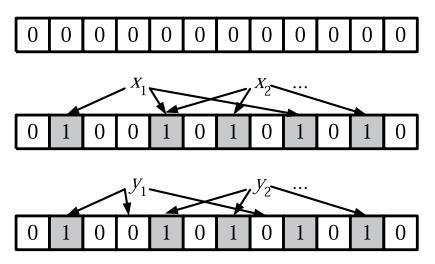
\includegraphics[width=0.55\linewidth]{image/BloomFilter}
	\caption[نمونه‌ای از عمکلرد فیلتر بلوم]{
		فیلتر مجموعه بدون عضو متشکل از یک آرایه‌ از بیت‌ها با مقدار صفر است. k دفعه چکیده هر عضو مجموعه $x_i$ محاسبه می‌شود که حاصل هر چکیده موقعیت یک بیت است. که مقدار این بیت‌ها ۱ می‌شود. حال برای آنکه بررسی کنیم که $y_i$ درون این مجموعه است به تعداد k بار از آن چکیده می‌گیریم و بیت‌های مرتبط را بررسی می‌کنیم. عنصر $y_1$ نمی‌تواند عضو مجموعه باشد چرا که یکی از بیت‌هایی که به آن اشاره می‌کند صفر است. عنصر $y_2$ یا عضو مجموعه است یا اینکه به خاطر خطای نوع دو فیلتر، عضو مجموعه تشخیص داده شده است.\cite{Broder2004}
	}
	\label{fig:bloomfilter}
\end{figure}

در فیلتر بلوم برای تنظیم نرخ قابل قبول خطای نوع دوم ($P_t$)، با توجه به حداکثر تعداد عناصری که در فیلتر قرار خواهند گرفت($M$)، اندازه فیلتر($n$) و تعداد توابع‌ چکیده‌ساز($k$) تعیین می‌شوند.
جدول \ref{table:BloomFilter} نشانه‌گذاری‌های مربوط به فیلتر بلوم را نشان می‌دهد.

\begin{table}[h]
	\centering
	\caption{قرارداد نشانه‌گذاری برای فیلتر بلوم}
	\label{table:BloomFilter}
	\begin{tabular}{|c|c|}
		\hline
		نشانه‌گذاری & معنا \\
		\hline
		\hline
		$\mathcal{S}$ & مجموعه عناصری که عضو فیلتر شده‌اند \\
		\hline
		$M$ & حداکثر تعداد عناصر فیلتر\\
		\hline
		$m = |\mathcal{S}|$ & تعداد عناصر قرار داده شده در فیلتر\\
		\hline
		$n$ & اندازه (تعداد بیت‌های) فیلتر \\
		\hline
		$k$ & تعداد توابع چکیده‌ساز\\
		\hline
		$\mathcal{U}$ & مجموعهٔ تمام عناصر، $|\mathcal{U}| = N_u$ \\
		\hline
		$\mathcal{V}$ & مجموعهٔ پنهان‌سازی (عناصر خطای نوع دو)، $|\mathcal{V}| = N_v$\\
		\hline
		$P_t$ & نرخ (احتمال) خطای نوع دوی هدف (ایده‌آل)\\
		\hline
		$P_f$ & نرخ (احتمال) خطای نوع دوی واقعی \\
		\hline
		$B(M, P_t)$ & فیلتر بلوم با حداکثر ظرفیت $M$ و نرخ خطای نوع دو هدف $P_t$ \\
		\hline
	\end{tabular}
\end{table}

برای فیلتر بلوم
$B(M, P_t)$
اندازه فیلتر به صورت زیر محاسبه می‌شود\cite{Gervais2014}:

\begin{equation}
n=-\frac{M\ln(P_t)}{\left(\ln(2)\right)^2} \label{eq:n_of_bloom_filter}
\end{equation}
و تعداد توابع چکیده‌ساز به صورت زیر محاسبه می‌گردد\cite{Gervais2014}:
\begin{equation}
k=\ln(2)\frac{n}{M} \label{eq:k_of_bloom_filter}
\end{equation}
احتمال خطای نوع دو فیلتر بلوم
$B(M, P_t)$
، در صورتی که $m$ عنصر در آن قرار دهیم که
$m<M$
، کمتر از مقدار هدف آن ($P_t$) می‌شود. اگر بیشتر از ظرفیت یک فیلتر در آن عنصر قرار داده شود،‌نرخ خطای نوع دو آن از از احتمال هدف بیشتر می‌گردد.

احتمال خطای نوع دو در یک فیلتر با توجه به عناصری که در آن قرار داده شده است، ($m$) با دقت‌های متفاوتی محاسبه شده است. مقاله \cite{Bloom1970}، که فیلتر بلوم را معرفی کرده است، احتمال خطای نوع دو را برای فیلتر بلوم محاسبه کرده است. این مقاله با فرض این‌که بعد از قرار دادن $m$ عضو در فیلتر بلوم نسبت بیت‌هایی که مقدار آن‌ها صفر مانده است به کل بیت‌ها برابر
$(1-k/n)^m$
باشد، احتمال خطای نوع دو را به صورت زیر محاسبه کرده است:

\begin{equation}
P_f(m) = \left(1-\left(1-\frac{k}{n}\right)^{m}\right)^k \label{eq:Pf_of_bloom_filter_Bloom}
\end{equation}

در مقاله \cite{Mullin1983} محاسبه دقیق‌تری از احتمال خطای نوع دو به دست آمده است. در این مقاله، احتمال آن که یک بیت دلخواه بعد از مقدار دهی k بیت مقدارش عوض نشود،
$(1-1/n)^k$
محاسبه شده است. پس به این ترتیب بعد از قرار دادن $m$ عضو در فیلتر، احتمال آن‌که مقدار یک بیت تغییر نکند، برابر 
$(1-1/n)^{km}$
خواهد بود. در نتیجه احتمال آن‌که مقدار یک بیت تغییر کند به صورت 
$p_{set} = 1-(1-1/n)^{km}$
محاسبه می‌شود. پس احتمال خطای نوع دو برابر است با احتمال آن‌که تمام بیت‌های انتخابی حاصل از $k$تا چکیدهٔ عنصری که عضو فیلتر بلوم مورد نظر نیست،‌ از قبل مقدار یک گرفته باشند. به این ترتیب احتمال خطای نوع دو طبق اثبات \cite{Mullin1983}، به صورت زیر محاسبه می‌شود.

\begin{equation}
P_f(m) = \left(1-\left(1-\frac{1}{n}\right)^{km}\right)^k \approx \left(1-e^{-\frac{mk}{n}}\right)^k
\label{eq:Pf_of_bloom_filter_Mullin}
\end{equation}

برای $n\gg k$، مقادیر معادله‌های  \eqref{eq:Pf_of_bloom_filter_Mullin} و \eqref{eq:Pf_of_bloom_filter_Bloom} به هم نزدیک خواهند بود. مقاله \cite{Christensen2010} به فرمولی با دقت بیشتر از دو مقاله قبلی برای محاسبه احتمال خطای نوع دوی فیلتر بلوم دست پیدا کرده است که به شرح زیر است:

\begin{equation}
P_f(m) = \frac{n!}{n^{k(m+1)}} \sum_{i=1}^{n} \sum_{j=1}^{i} (-1)^{i-j} \frac{j^{km}i^k}{(n-i)!j!(i-j)!}
\label{eq:Pf_of_bloom_filter_Christensen}
\end{equation}


اثبات فرمول \eqref{eq:Pf_of_bloom_filter_Christensen} خارج از بحث این پایان‌نامه است. اگر تعداد پیام‌های قرارداده شده در فیلتر بلوم برابر با $M$ باشد، در آن صورت 
$P_f(M)=P_t$.


کاربرد‌های متعددی برای فیلتر بلوم وجود دارد و در ادامه یکی از آن‌ها را مرور خواهیم کرد. در وبسایت‌هایی که خدمات کوتاه‌کردن لینک را ارائه می‌کنند (مانند \cite{Bitly.comTeam2020})، معمولا لیست سیاهی از آدرس‌های غیر امن نگهداری می‌شود و به کاربر استفاده کننده از لینک‌های کوتاه‌شده اطمینان می‌دهد که آدرسی که به آن هدایت خواهد شد یک آدرس امن است (در لیست سیاه آدرس‌های ناامن قرار ندارد). جست‌وجو کردن لیست سیاه آدرس‌های ناامن برای هر درخواست امری زمان‌بر است. از این رو، مجموعهٔ تمام آدرس‌های ناامن در یک فیلتر بلوم نگهداری می‌شود. اگر پاسخ فیلتر بلوم برای یک آدرس درخواست داده شده منفی باشد (عضو مجموعه نباشد) می‌توانیم صددرصد مطمئن باشیم که آدرس در‌خواست داده شده یک آدرس امن است و اگر پاسخ مثبت باشد،‌ جهت جبران خطای نوع دو، پایگاه‌ داده لیست سیاه آدرس‌های ناامن را جست‌وجو می‌کند\cite{Azar2016}.

کاربرد فیلتر بلوم مورد نظر در این پایان‌نامه، استفاده از آن در گره‌های سبک برای حفظ گم‌نامی این گره‌ها است \cite{Hearn2013}. در بخش‌  \ref{BloomFilterInP2P} به نحوهٔ استفاده از این فیلتر در ارتباط بین گره‌های سبک و گره‌های کامل پرداخته می‌شود و در بخش \ref{Vulnerabilities} به ضعف‌ها و آسیب‌پذیری‌های استفاده از این فیلتر در شبکه بیت‌کوین خواهیم پرداخت. 


\subsection{فیلتر بلوم در شبکهٔ همتا‌به‌همتای بیت‌کوین}
\label{BloomFilterInP2P}

امکان استفاده از فیلتر بلوم در ارتباط بین گره سبک و گره کامل به دنبال معرفی آن در طرح پیشنهادی بهبود بیت‌کوین شمارهٔ ۳۷ (\lr{BIP37}) \cite{Hearn2013} در سال ۲۰۱۳ فراهم شد.  گره‌‌های سبک برای حفظ گم‌نامی خود، به جای آن‌که آدرس‌های مربوط به خودشان را صورت فاش در اختیار یک گره کامل قراردهند، آدرس‌های خود و دیگر اطلاعات مورد نیازشان را در یک فیلتر بلوم با نرخ خطای نوع دوی معین قرار می‌دهند. گره کامل با تطابق داده‌های داخل تراکنش‌ها با فیلتر بلوم بررسی می‌کند آن داده درون فیلتر بلوم صدق می‌کند یا خیر. اگر یک داده درون فیلتر بلوم صدق کرد، گره کامل آن داده را برای گره سبک ارسال می‌کند. به صورت کلی اطلاعاتی که می‌توانند درون فیلتر بلوم قرار بگیرند و توسط گره کامل با فیلتر بلوم تطابق داده می‌شوند می‌شوند به صورت زیر است:
\begin{enumerate}
\item{%
چکیدهٔ تراکنش‌ (\lr{TXID})}
\item{%
برای هر خروجی تراکنش، داده‌های
%نبشتهٔ\RTLfootnote{Script} 
\gls{Script}
خروجی بررسی می‌شوند. این داده‌ها نظیر \lr{pubKeyHash} یا \lr{pubKey} هستند. زمانی که یکی از این داده‌ها با فیلتر بلوم تطابق پیدا کنند، گره کامل، در صورت درخواست کاربر، مintی‌تواند دادهٔ \lr{COutPoint} را به فیلتر اضافه نماید. به این‌ترتیب فیلتر را به‌روزرسانی کند.
}
\item{%
برای هر ورودی، \lr{COutPoint} بررسی می‌شود.
}
\item{%
برای هر ورودی، داده‌های نبشتهٔ ورودی بررسی می‌شوند. این داده‌ها نظیر 
\lr{pubKey}
یا
\lr{sig} 
هستند.
}
\end{enumerate} 

اگر گره‌کامل بتواند در یک تراکنش مطابقتی بین هر کدام از موارد بالا و فیلتر بلوم پیدا کند آن تراکنش را برای گره سبک ارسال می‌کند. در غیر این صورت چیزی برای گره سبک ارسال نمی‌شود. در ادامه، به بررسی پروتکل ارتباطی گره‌های سبک با گره‌های کامل و گرفتن اثبات مرکل  برای تراکنش‌های مورد نظر کاربر سبک با بهره‌گیری از فیتلر بلوم پرداخته خواهد شد. 

در قسمت \ref{P2PNetwork}، نحوهٔ اتصال یک گره سبک به گره‌های فعال شبکه‌ٔ همتا‌به‌همتای بیت‌کوین توضیح داده شد. در این قسمت نحوهٔ ساخت و فرستادن فیلتر بلوم به یک گره کامل و دریافت تراکنش‌های موجود در یک بلوک که در آن فیلتر صدق می‌کنند پرداخته خواهد شد.

\subsubsection{ساخت فیلتر بلوم}
همان‌طور که در بخش \ref{BloomFilter} توضیح داده‌شد، فیلتر بلوم دو پارامتر تعیین‌کننده دارد: اندازهٔ (تعداد بیت‌های) فیلتر ($n$) و تعداد توابع چکیده‌ساز فیلتر ($k$). قطعه کد زیر از فایل \lr{BloomFilter.java} از منبع کد بیت‌کوین‌جی \cite{bitcoinj_BloomFilter} نحوه‌ٔ اختصاص‌دهی مقادیر $n$ و $k$ را که به ترتیب با متغیر‌های \texttt{size} و \texttt{hashFuncs} مشخص شده‌اند و طبق فرمول‌های \eqref{eq:n_of_bloom_filter} و \eqref{eq:k_of_bloom_filter} محاسبه شده‌اند نشان می‌دهد:

\lr{
%\begin{flushleft}
	\texttt{int size = (int)(-1/(pow(log(2),2))*elements*log(falsePositiveRate));\\
size = max(1,min(size,(int)MAX\_FILTER\_SIZE*8)/8);\\
hashFuncs = (int)(data.length*8/(double)elements*log(2));\\
hashFuncs = max(1,min(hashFuncs,MAX\_HASH\_FUNCS));\\
}
%\end{flushleft}	
}

اندازه فیلتر بلوم حداکثر می‌تواند $36000$ بایت (\lr{``MAX\_FILTER\_SIZE''}) و تعداد توابع چکیده‌ساز حداکثر می‌تواند $50$ (\lr{``MAX\_HASH\_FUNCS''}) باشد. در فیلتر بلوم بیت‌کوین از نسخهٔ ۳ تابع چکیده‌ساز ۳۲ بیتی 
مورمور \LTRfootnote{\lr{MurmurHash3 (x86\_32)}}
استفاده می‌شود\cite{Hearn2013}. برای دستیابی به $k$ تابع چکیده‌ساز متفاوت، از مقدار 
%بذر \RTLfootnote{Seed}
\gls{Seed}
متفاوتی برای هرکدام از توابع استفاده می‌شود. بذر هر تابع چکیده‌ساز مطابق فرمول \eqref{eq:Bloom_hash_seed} محاسبه می‌شود.

\begin{equation}
\label{eq:Bloom_hash_seed}
SEED_{(nHashNum)} = nHashNum \times \text{\lr{0xfba4c795}} + nTweak
\end{equation}
که در آن \lr{nHashNum}، شمارهٔ ترتیب تابع چکیده‌ساز است. مقدار آن برای اولین تابع چکیده‌ساز صفر و برای آخرین تابع $k-1$ است. عدد \lr{0xfba4c795} یک عدد ثابت بهینه‌شده است تا اختلاف مقدار بذر توابع مختلف را زیاد نماید. \lr{nTweak} به ازای هر فیلتر بلوم مقدار متفاوتی دارد که توسط کاربر سبک انتخاب می‌شود. 

سپس برای تعیین بیت‌هایی که باید در فیلتر بلوم مقدار آن‌ها به یک تغییر کند، چکیدهٔ هر کدام از آدرس‌های مورد نظر را توسط هر $k$ تابع چکیده‌ساز حساب کرده و باقیمانده‌ حاصل را به اندازهٔ فیلتر بلوم می‌سنجیم. حاصل شماره بیتی است که باید اندازه‌ٔ آن به یک تغییر بکند. دستور محاسبهٔ چکیده در فایل \lr{bloom.cpp} هسته‌ٔ بیت‌کوین در کد منبع آن \cite{Bitcoincore.org}به صورت زیر است:

\lr{
%	\begin{flushright}
		\texttt{MurmurHash3(nHashNum*0xFBA4C795+nTweak, vDataToHash)\%(vData.size()*8)
		}
%	\end{flushright}	
}




\subsubsection{فرستادن فیتلر بلوم برای گره کامل}

بعد از آن‌که گره سبک باتوجه به مقادیر مورد نظرش فیلتر بلوم را تولید کرد، لازم است که آن را از طریق پیام \texttt{filterload} برای گره کامل ارسال نماید. به این ترتیب کاربر سبک می‌تواند تراکنش‌هایی که مربوط به کیف پولش هستند به علاوهٔ تعدادی تراکنش حاصل از خطای نوع دو دریافت نماید تا مانع اطلاع گره کامل از آدرس‌های مربوط به گره سبک شود. جدول  \ref{table:filterloadMessage} قسمت‌های مختلف پیام \texttt{filterload} را توضیح می‌دهد.

\begin{xltabular}{\textwidth}{|c|X|}
	\caption{
		قسمت‌های پیام \texttt{filterload} در شبکه همتا‌به‌همتای بیت‌کوین
		\label{table:filterloadMessage}}\\
	\hline
	\textbf{نام} & {\textbf{توضیحات}} \\
	\hline \hline
	\lr{nFilterBytes} &{%
تعداد بایت‌های فیلتری که در قسمت بعدی قرار گرفته است.	
}\\
\hline
	\lr{filter} &{%
	آر‌ایه از بیت‌ها که همان فیلتر بلوم است. حداکثر اندازهٔ آن می‌تواند $36000$ باشد.
}\\
\hline
	\lr{nHashFuncs} &{%
	تعداد توابع چکیده‌ساز به‌کار گرفته‌شده در فیلتر بلوم. حداکثر تعداد آن می‌تواند $50$ باشد.
}\\
\hline
	\lr{nTweak} &{%
	یک مقدار دلخواه برای اضافه کردن بذر به توابع چکیده‌ساز استفاده شده در فیلتر بلوم. عملا گره دریافت‌کنندهٔ این پیام می‌تواند با استفاده از این مقدار تمام توابع چکیده‌ساز مورد نیاز را ایجاد نماید.
}\\
\hline
	\lr{nFlags} &{%
	این بخش می‌تواند یکی از مقادیر زیر را داشته باشد. هر کدام از این مقادیر به گره کامل می‌گوید که در آینده چه تغییراتی در فیلتر بلوم ارسال شده ایجاد نماید.
}\\
&{%
۱- صفر (\lr{BLOOM\_UPDATE\_NONE}): گره کامل نباید تغییری در فیلتر بلومی که در اختیار دارد ایجاد نماید.
}\\
&{%
۲- یک (\lr{BLOOM\_UPDATE\_ALL}): اگر فیلتر با هر یک از داده‌های نبشتهٔ خروجی تطابق پیدا کند، گره کامل \lr{COutPoint} را به فیلتر اضافه نماید و فیلتر را به‌روزرسانی کند.
}\\
&{%
	۳- دو (\lr{BLOOM\_UPDATE\_P2PUBKEY\_ONLY}): اگر فیلتر با هر یک از داده‌های نبشتهٔ خروجی تطابق پیدا کند، تنها اگر نبشته از نوع \lr{P2PK} یا \lr{P2SH} باشد، گره کامل \lr{COutPoint} را به فیلتر اضافه نماید و فیلتر را به‌روزرسانی کند.
}\\
&{%
	از آن‌جایی که گره کامل با توجه به تطبیق‌های اشتباهی که به خاطر خطای نوع دو انجام شده است نیز فیلتر بلوم را به روزرسانی می‌کند، عناصر موجود در فیلتر بلوم بسیار سریع زیاد خواهد شد و به خاطر بالا رفتن نرخ خطای نوع دو خیلی زود فیلتر بلااستفاده خواهد شد.
}\\
\hline
	
\end{xltabular}

گره سبک می‌تواند با فرستادن پیام \texttt{filterclear} به گره دریافت‌کننده بگوید که فیلتر بلومی که قبل‌تر برایش ارسال شده است را پاک کند. پیام \texttt{filterclear} هیچ پایه‌باری ندارد و برای آن‌که گره سبک یک فیلتر بلوم جدید ارسال نماید، نیاز نیست که فیلتر بلوم قبلی را حذف کند. گره سبک همچنین می‌تواند با فرستادن پیام \texttt{filteradd} به گره دریافت کننده، داده‌ای را به فیلتر بلومی که پیش‌تر برایش ارسال کرده بوده اضافه نماید. بدون آن که نیازی باشد که یک فیلتر بلوم جدید را برای او ارسال کند. به ‌این ترتیب،‌ از آنجایی که عنصر جدید مستقیما به گره دریافت کننده ارسال می‌شود، حریم خصوصی کاربر حفظ نمی‌شود. از این رو کاربر برای حفظ نسبی حریم خصوصیش باید مجددا فیلتر بلوم جدید را محاسبه کند و به وسیلهٔ پیام \texttt{filterload} برای گره کامل ارسال نماید.


به این ترتیب گره سبک سعی می‌کند که به جای ارسال مستقیم آدرس‌هایش به یک گره کامل، آدرس‌هایش را درون یک فیلتر بلوم قرار دهد و این فیلتر با با پیام \texttt{filterload} برای یک گره کامل ارسال نماید. گره کامل عناصر متفاوتی از یک تراکنش را در فیلتر بلوم ارسال شده ارزیابی می‌کند و همچنین می‌تواند در صورت اجازهٔ گره سبک آن را به روزرسانی نماید.

\subsubsection{اطلاعات دریافتی به ازای هر تراکنش منطبق شده}
همان‌طور که در بخش \ref{P2PNetwork} شرح داده شد، گره سبک بعد از آن‌که برای بار اول فیلتر بلوم را با گره(های) هم‌گام‌ساز به اشتراک گذاشت، به ازای هر بلوک جدیدی که از شبکهٔ همتا‌به‌همتا به گره(های) هم‌گام‌ساز می‌رسید، از طرف آن‌(ها) به گره سبک یک پیام \texttt{inv} ارسال می‌شد. گره سبک بعد از دریافت این پیام، یک پیام \texttt{getdata} برای آن‌ها ارسال می‌کرد و به این طریق از آن‌ها می‌خواست که داده‌های تراکنش‌ها را با فیلتر بلوم ارسالی ارزیابی کنند و اگر داده‌ای از یک تراکنش با آن فیلتر مطابق شد، آن تراکنش را به علاوهٔ اثبات مرکل برای آن گره سبک ارسال کنند.

گره‌های کامل تراکنش‌های منطبق شده را در قالب پیام \texttt{tx}، که پایه‌بار آن یک تراکنش خام است، برای گره سبک ارسال می‌کنند. علاوه بر آن پیام \texttt{merkleblock} که شامل \lr{TXID}های تراکنش‌ها و هر بخشی از درخت مرکل که نیاز است که این تراکنش‌ها را به ریشهٔ مرکل موجود در سرایند بلوک مرتبط کند، است. بخش‌های پیام \texttt{merkleblock} در جدول  \ref{table:merkleblockMessage} شرح داده شده‌اند.

\begin{xltabular}{\textwidth}{|c|X|}
	\caption{
		قسمت‌های پیام \texttt{merkleblock} در شبکه همتا‌به‌همتای بیت‌کوین
		\label{table:merkleblockMessage}}\\
	\hline
	\textbf{نام} & {\textbf{توضیحات}} \\
	\hline \hline
	\lr{block header} & {%
سرایند بلوکی که تراکنش‌ها از آن انتخاب شده‌اند و اثبات مرکل مرتبط در این پیام قرار داده شده‌ است.	
}\\
\hline

	\lr{transaction count} & {%
	تعداد کل تراکنش‌های موجود در بلوک انتخابی.
}\\
\hline

	\lr{hash count} & {%
	تعداد چکیده‌های موجود در قسمت بعدی.
}\\
\hline

	\lr{hashes} & {%
	شامل چکیده‌ٔ تراکنش‌ها (\lr{TXID}) و گره‌های درخت مرکل است.
}\\
\hline

	\lr{flag byte count} & {%
	تعداد بایت‌های پرچمی که در قسمت بعدی آمده است.
}\\
\hline

	\lr{flags} & {%
مجموعه‌ای از بیت‌ها که که هرکدام از چکیده‌ها را به یک گره در درخت مرکل اختصاص می‌دهند. نحوهٔ عملکرد آن در مثالی در متن آورده شده است. تعداد بیت‌های آن باید به هشت (اندازهٔ یک بایت) بخش‌پذیر باشد. برای این منظور می‌شود از لایی‌گذاری صفر استفاده کرد.
}\\
\hline
\end{xltabular}

\paragraph{مثال}
در این مثال فرض کنید که پیام \texttt{merkleblock} بدون سرایند مطابق زیر باشد \cite{P2P_ref}:

\lr{%
\texttt{%
01000000 ........................... Block version: 1\\
82bb869cf3a793432a66e826e05a6fc3\\
7469f8efb7421dc88067010000000000 ... Hash of previous block's header\\
7f16c5962e8bd963659c793ce370d95f\\
093bc7e367117b3c30c1f8fdd0d97287 ... Merkle root\\
76381b4d ........................... Time: 1293629558\\
4c86041b ........................... nBits: 0x04864c * 256**(0x1b-3)\\
554b8529 ........................... Nonce\\
\newline
07000000 ........................... Transaction count: 7\\
04 ................................. Hash count: 4\\
\newline
3612262624047ee87660be1a707519a4\\
43b1c1ce3d248cbfc6c15870f6c5daa2 ... Hash \#1\\
019f5b01d4195ecbc9398fbf3c3b1fa9\\
bb3183301d7a1fb3bd174fcfa40a2b65 ... Hash \#2\\
41ed70551dd7e841883ab8f0b16bf041\\
76b7d1480e4f0af9f3d4c3595768d068 ... Hash \#3\\
20d2a7bc994987302e5b1ac80fc425fe\\
25f8b63169ea78e68fbaaefa59379bbf ... Hash \#4\\
\newline
01 ................................. Flag bytes: 1\\
1d ................................. Flags: 1 0 1 1 1 0 0 0\\}}

با استفاده از تعداد تراکنش‌ها گره سبک می‌تواند یک درخت مرکل خالی را ایجاد نماید. در این مثال که تعداد تراکنش‌ها هفت است، درخت مرکل سه لایه خواهد داشت. در اثبات مرکل اگر گره کامل چکیدهٔ یک گره مرکل را در اختیار کاربر سبک قرار دهد، کاربر سبک می داند که دیگر از گره‌ها یا \lr{TXID}های زیردستی آن مقداری در اختیار وی قرار نداده است. ترتیب چکیده‌ها و بیت‌های \lr{flags} یکی است. شروع حرکت از ریشهٔ درخت مرکل است و برای حرکت به سمت گره‌های بچه، ابتدا گره چپ را انتخاب می‌کنیم. اطلاعات زیر را می‌توانیم با توجه به \lr{flags} راجع به جایگاه مقادیر چکیده در درخت مرکل بدست بیاوریم:
\begin{enumerate}
	\item{%
	\textbf{مقدار صفر:}
	به این معنی است که اولین مقدار چکیدهٔ استفاده نشده را به عنوان مقدار این گره استفاده کن و گره‌های پایین دستی این گره را رها کن. به اولین گرهی برو که مقدار آن محاسبه نشده است.
}
	\item{%
	\textbf{مقدار یک:}
	مقدار چکیدهٔ این گره نیاز به محاسبه شدن دارد. برای این منظور گره بعدی را گره بچهٔ سمت چپی قرار بده اما اگر مقدار چکیده در گره بچهٔ سمت چپ محاسبه شده است به گره بچهٔ سمت راست برو.
}
\end{enumerate}

\begin{figure}
	\centering
	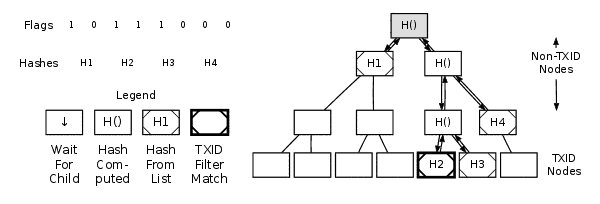
\includegraphics[width=\linewidth]{image/merkleblock-parsing}
	\caption{شکل مثال تحلیل پیام \texttt{merkleblock} در سمت کاربر سبک.\cite{P2P_ref}}
	\label{fig:merkleblock-parsing}
\end{figure}

با توجه به توضیحات بالا، گام‌های محاسبهٔ اثبات مرکل با توجه به پیام \texttt{merkleblock} دریافت شده در مثال به صورت زیر خواهد بود:

\begin{enumerate}
		\item {%
		باتوجه به اینکه تعداد تراکنش‌ها هفت عدد است، یک درخت مرکل سه لایه، مطابق شکل \ref{fig:merkleblock-parsing} ایجاد می‌کنیم که در ابتدا تمام گره‌های آن خالی باشد.
	}
	\item {%
		از ریشهٔ مرکل شروع می‌کنیم. مقدار اولین بیت \lr{flags} یک است. به این ترتیب مقدار گره ریشه بعدا و با توجه به مقدار بچه‌هایش مشخص می‌شود. گره بعدی مورد بررسی را بچهٔ سمت چپ ریشهٔ مرکل قرار می‌دهیم. برای شماره گذاری، گره ریشه را گره شمارهٔ یک می‌نامیم.
	}

	\item {%
در این مرحله، گره مورد بررسی گره بچهٔ سمت چپ ریشهٔ مرکل است. با توجه به اینکه بیت بعدی \lr{flags} برابر صفر است، اولین چکیدهٔ استفاده نشده (\lr{Hash \#1}) را در این گره قرار می‌دهیم و دیگر کاری با گره‌های زیر دستی آن داریم. این گره را گره شمارهٔ دو می‌نامیم. به این ترتیب مطابق شکل \ref{fig:merkleblock-parsing} مقدار \lr{H1} در این گره قرار می‌گیرد. به گره بالاتر (ریشهٔ مرکل) برگشته و بچهٔ راستی آن را انتخاب می‌کنیم.
	}
	\item{%
	شماره این گره را سه می‌گذاریم. مقدار بیت بعدی (سوم) \lr{flags} برابر ۱ است، پس  مقدار این گره باید توسط گره‌های زیردستی آن محاسبه شود. به این ترتیب، بچهٔ سمت چپی آن انتخاب می‌شود. 
}
	\item{%
	شمارهٔ این گره را چهار می‌گذاریم. در این مرحله‌ هم مانند مرحلهٔ قبل، چون بیت چهارم \lr{flags} نیز یک است گره بچهٔ سمت چپی انتخاب می‌شود.
}
	\item{%
	شمارهٔ این گره را پنج می‌نامیم. در این مرحله یک گره \lr{TXID} انتخاب شده است. از آن‌جا که گره‌های مربوط به تراکنش‌ها زیرگره‌ای ندارند، مقدار آن‌ها حتما باید توسط گره کامل در اختیار گره سبک قرار گیرد. به این ترتیب مقدار چکیدهٔ استفاده نشدهٔ بعدی، یعنی \lr{Hash \#2} را در این گره قرار می‌دهیم. مقدار بیت پنجم \lr{flags} که متناظر با این گره است برابر یک بوده که این معنا را می‌رساند که این \lr{TXID} برای تراکنشی است که یکی از عناصر آن با فیلتر بلوم منطبق شده‌اند پس به گره سبک دریافت کننده مربوط است. 
}

	\item{%
	در مرحلهٔ بعدی، به گره پدر (چهارم) برگشته و گره بچهٔ سمت راستی انتخاب می‌شود. این گره، گره ششم است. باز هم چون این گره، بچه‌ای ندارد و مربوط به یک \lr{TXID} است، مقدار  \lr{Hash \#3} را در آن قرار می‌دهیم. بیت ششم \lr{flags} صفر بوده به این معنا است که این تراکنش با فیلتر منطبق نشده است. ارسال آن صرفا برای اثبات مرکل نیاز است.
}

	\item{%
	به گره پدر (گره چهارم) بر می‌گردیم. از آن‌جایی که اطلاعات لازم برای محاسبهٔ چکیدهٔ این گره را از دو مقدار  \lr{TXID} داده شده داریم، مقدار چکیدهٔ را محاسبه کرده و سپس گره بالاتر را انتخاب می‌کنیم. 
}
	\item{%
	در این مرحله وارد بچهٔ راست سومین گره می‌شویم. چون مقدار بیت هفتم \lr{flags} صفر است، چکیدهٔ \lr{Hash \#4} را درون آن قرار می‌دهیم. در این مرحله دیگر گره‌ای نیست که گره کامل مقدار آن را فرستاده باشد و بیت آخر \lr{flags} به خاطر لایی گذاری مقدار صفر دارد. 
}
	\item{%
	در مرحلهٔ آخر مقدار چکیدهٔ گره سوم و به تبع آن مقدار ریشهٔ درخت مرکل را محاسبه می‌کنیم. بررسی می‌شود که مقدار ریشهٔ محاسبه شده با مقدار ریشهٔ مرکلی که در سرایند بلوک قرار داشته است یکسان باشد.
}
\end{enumerate}


\subsubsection{ملاحظات پیاده‌سازی}
بیت‌کوین‌جی\cite{bitcoinj} به صورت پیش‌فرض، نرخ خطای نوع دو را برابر $0.1$ درصد قرار می‌دهد. هرچند که بالا بردن نرخ خطای نوع دو می‌تواند به حفظ بهتر حریم خصوصی کاربران سبک بیانجامد اما نه تنها باعث افزایش پهنای باند مصرفی کاربر سبک می‌شود، بلکه احتمال آن که آدرس‌های پر استفاده‌ای مثل 
ساتوشی‌دایس\LTRfootnote{%
	\lr{Satoshi Dice (\url{https://satoshidice.com/})} - %
سایت ساتوشی‌دایس درحال حاضر تنها از بیت‌کوین‌کش پشتیبانی می‌کند!}،
که یک سایت شرط‌بندی مبتنی بر زنجیرهٔ بلوکی است، منطبق با فیلتر بلوم شود بیشتر خواهد شد. در این صورت اطلاعات به شدت زیادی برای کاربر سبک ارسال خواهد شد و اگر کاربر سبک به گره کامل هم‌گام‌ساز اجازه دهد که فیلتر را به‌روز رسانی کند، به سرعت فیلتر اشباع و بلااستفاده خواهد شد.
 
در کتاب‌خانهٔ بیت‌کوین‌جی، اگر کاربر بخواهد $m$ عنصر را در فیلتر بلوم قرار دهد، مقادیر اندازه فیلتر ($n$) و تعداد توابع چکیده‌ساز آن ($k$) با توجه به $100$ عنصر اضافه‌تر طبق فرمول‌های \eqref{eq:n_of_bloom_filter} و \eqref{eq:k_of_bloom_filter} تعیین می‌شوند 
$M=m+100$ \cite{Gervais2014}.
 هدف از این کار آن است که امکان اضافه شدن عناصر جدید به فیلتر بلوم توسط خود کاربر یا توسط گره کامل، بدون نیاز به به‌روزرسانی آن مطابق آن‌چه قبل‌تر توضیح داده شد، فراهم باشد به نحوی که فیلتر بلوم سریع پر نشود و نرخ خطای نوع دو آن به قدری زیاد نشود که فیلتر بلوم عملا بلااستفاده شود. در حالی که به مرور زمان به تعداد عناصر فیلتر بلوم یک کاربر SPV اضافه می‌شود، قاعدتا، مقادیر $k$ و $n$ تغییری نمی‌کنند. اما اگر کاربر SPV نیاز به راه‌اندازی مجدد کیف‌پولش داشته باشد، در راه‌اندازی دوباره، نرم‌افزار بیت‌کوین‌جی با توجه به $m$، جدید، اقدام به محاسبهٔ $M=m+100$ می‌نماید و به این ترتیب مقادیر  $k$ و $n$ برای فیلتر جدید متفاوت خواهند بود.
 
همچنین در پیاده‌سازی گره سبک بیت‌کوین‌جِی برای هر آدرس، کلید عمومی (\lr{PubKey}) و چکیدهٔ کلید عمومی (\lr{PubKeyHash}) گذاشته می‌شود. پس به ازای یک آدرس بیت‌کوین، دو عنصر در فیلتر بلوم قرار می‌گیرند. به بیان دیگر، در ازای قرار دادن $N$ آدرس در فیلتر بلوم، $m=2N$ عنصر در آن قرار می‌گیرد پس با توجه به آن‌چه در بالا گفته شد، می‌توان نوشت $M=2N+100$. قرار دادن کلید عمومی و چکیدهٔ آن یک آسیب‌پذیری در فیلتر بلوم ایجاد خواهد کرد که به گره متخاصم این امکان را می‌دهد که در صورتی که متوجه شود یک \lr{PubKey} در فیلتر بلوم قرار دارد، مقدار چکیده (\lr{PubKeyHash}) آن  را نیز امتحان می‌کند. اگر مقدار چکیده هم در فیلتر بلوم قرار داشت، با اطمینان بیشتری می‌تواند مطمئن شود که این آدرس، یکی از آدرس‌های کاربر سبکِ استفاده کننده از فیلتر بلوم است. قطعه کد زیر بخشی از پیاده‌سازی فیلتر بلوم در کد بیت‌کوین‌جِی است \cite{bitcoinj_BloomFilter} که این مسئله را به خوبی نشان می‌دهد.


\lr{
	\texttt{/** Inserts the given key and equivalent hashed form (for the address). */\\
		public synchronized void insert(ECKey key) \{\\
		insert(key.getPubKey());\\
		insert(key.getPubKeyHash());\\
		\}\\}
}


در پایان‌نامهٔ\cite{Nick2015}، با هدف پیدا کردن آدرس‌های نهفته شده در این فیلتر بلوم با استفاده از این آسیب‌پذیری، در بازهٔ تاریخی $12$ دسامبر $2014$ الی $10$ فوریه $2015$، یک گره کامل راه‌اندازی شده و شروع به جمع‌آوری $70,078$ فیلتر بلوم از کاربران سبک کرده است. همچنین، در این پایان‌نامه، مجموعه‌ای از تمام کلید عمومی‌ها (\lr{PubKey}) و چکیدهٔ کلید عمومی (\lr{PubKeyHash}) متناظر آن‌ها که در زنجیرهٔ بلوکی مورد استفاده قرار گرفته‌اند جمع‌آوری شده است. در نهایت همهٔ آن‌ها را با تمام فیلتر‌های بلوم جمع شده تطبیق داده است. اگر هر جفت کلید عمومی و چکیدهٔ آن بر فیلتر منطبق بود، نتیجه گرفته است که آن آدرس در آن فیلتر قرار دارد. در نهایت این پایان‌نامه توانسته است به $55,111$ جفتِ کلید عمومی و چکیدهٔ آن برسد که هردو در یک فیلتر بلوم منطبق هستند.

هرچند که این ایراد به نظر ایرادی می‌آید که به سادگی قابل حل شدن باشد، اما در صورتی که بیت‌کوین‌جی کلید عمومی‌ها را در فیلتر قرار ندهد، کیف پول‌هایی که از آن کتاب‌خانه استفاده می‌کنند نخواهند توانست از تراکنش‌هایی که خروجی آن‌ها \lr{P2PK} است مطلع شود. در حالی که، بیت‌کوین‌جی می‌خواهد از تمام انواع تراکنش‌ها پشتیبانی کند. به خاطر همین، باتوجه به آگاهی به وجود این مشکل، اقدامی برای برطرف کردن آن انجام نشده است.

در کنار مشکلات ذکر شده، استفاده از فیلتر بلوم در شبکهٔ همتا‌به‌همتای بیت‌کوین با آسیب‌پذیری‌ها و چالش‌های بیشتری مواجه است که عملا این ابزار را برای حفظ حریم خصوصی کاربران سبک بلااستفاده کرده است. در بخش \ref{Vulnerabilities} به بررسی این ضعف‌ها پرداخته شده است.

\subsubsection{آسیب‌‌پذیری‌ها }
\label{Vulnerabilities}
مقالهٔ \cite{Gervais2014} به طور مفصل به بررسی آسیب‌پذیری‌های موجود در فیلتر بلوم استفاده شده در شبکهٔ همتا‌به‌همتای بیت‌کوین پرداخته است. در این مقاله توضیح داده شده است که فیلتر بلوم نشت اطلاعاتی بسیار زیادی دارد که این نشت به تعداد آدرس‌هایی که یک کاربر دارد وابسته است. اگر کاربر تعداد متوسطی، مثلا $10$ آدرس، را در فیلتر بلومی قرار دهد، مهاجم می‌تواند با احتمال خوبی آدرس‌های قرار گرفته شده در فیلتر بلوم را حدس بزند. به عنوان مثال احتمال درست حدس زدن آدرس‌های فیلتر بلوم با $10$ آدرس برابر $0.99$ است.  

علاوه بر این حتی اگر تعداد آدرس‌ها در فیلتر‌ بلوم افزایش پیدا کند، در حالی که مهاجم بتواند به دو فیلتر بلوم مربوط به یک کاربر سبک دست پیدا کند، قادر خواهد بود که با دقت بالایی آدرس‌های مربوط به کاربر سبک را تشخیص دهد. چرا که اگر یک گره کامل متخاصم دو فیلتر بلوم متفاوت از یک کیف پول را در دست داشته باشد، می‌تواند با وارد کردن عناصر به هر دو فیلتر، تا حد قابل ملاحظه‌ای خطاهای نوع دوم را برطرف نماید\cite{Nick2015}. لازم به ذکر است که در پیاده‌سازی‌های فعلی با راه‌اندازی مجدد گره سبک، چون از مقدار تصادفی \lr{nTweak} متفاوتی استفاده خواهد شد، فیلتر بلوم تغییر می‌کند و به گره کامل متخاصم شانس دسترسی به فیلتری‌های بلوم متعددی از یک کاربر سبک را می‌دهد\cite{Gervais2014} .

در مقالهٔ \cite{Gervais2014}، به معرفی یک معیار برای سنجش حریم خصوصی  فیلتر بلوم پرداخته است. این معیار اینطور تعریف می‌شود که 
$P_{h_{(j)}}$
 برابر است با احتمال آن‌که یک گره متخاصم، ‌$j$ عنصری که واقعا در فیلتر بلوم قرار گرفته‌اند و فرد متخاصم اطلاعاتی در مورد آن‌ها نداشته است را درست حدس بزند. محاسبهٔ $P_{h_{(j)}}$ به صورت زیر است:
%N_v = S
 \begin{equation}
 \label{eq:P_h}
 P_{h_{(j)}} = \prod_{k=0}^{j-1}\frac{N-k}{N+N_v-k} = \frac{N}{N+N_v}\cdot\frac{N-1}{N+N_v-1} \ldots
 \end{equation}
  
  که در آن $N$ تعداد آدرس‌هایی است که در بیت‌کوین قرار داده شده است. از آن‌جایی که هم \lr{PubKey} و هم \lr{PubKeyHash} درون فیلتر بلوم قرار می‌گیرند، تعداد عناصر قرار گرفته در فیلتر بلوم برابر $m=2N$ است. $N_v$ هم تعداد اعضای مجموعه‌ٔ عناصری است که به خاطر خطای نوع دو با فیلتر بلوم منطبق می‌شوند. از نظر شهودی، معادلهٔ \eqref{eq:P_h} به معنی احتمال آن است که $j$ آدرس انتخاب شده از بین تمام آدرس‌هایی که منطبق با فیلتر بلوم می‌شوند، جزء آدرس‌های اصلی فیلتر باشند.
  
   با توجه به معادلهٔ \eqref{eq:P_h} احتمال آن‌که کاربر متخاصم تمام آدرس‌هایی که در حقیقت درون فیلتر بلوم $B$ هستند را به درستی حدس بزند، برابر 
  $P_{h_{(N)}} = \prod_{k=0}^{N-1}\frac{N-k}{N+N_v-k} = \frac{N!N_v!}{(N+N_v)!}$
  خواهد بود\cite{Gervais2014}. بدیهی است که هر چه مقدار $P_{h_{(.)}}$ بیش‌تر باشد،‌ فیلتر بلوم حریم خصوصی را کمتر حفظ می‌کند. علاوه بر این گره کامل می‌تواند تعداد عناصر قرارداده شده در فیلتر را نیز حدس بزند که این خود می‌تواند به برملاء شدن اطلاعات کاربر کمک نماید. در این مقاله با فرض این‌که گره کامل متخاصم تنها بتواند به یک فیلتر بلوم مربوط به یک کیف پول دسترسی پیدا کند، می‌تواند تخمینی از تعداد عناصر موجود در یک فیلتر بلوم را با توجه به اندازهٔ فیلتر، توابع چکیده‌ساز و تعداد بیت‌هایی از فیلتر که یک شده‌اند انجام دهد. این مقاله این تخمین را با بهره‌گیری از ایدهٔ مقالهٔ \cite{Swamidass2007} محاسبه کرده است که به شرح زیر است:
  
   \begin{equation}
  \label{eq:m_estimation}
 m \approx -n\frac{\ln\left(1-\frac{X}{n}\right)}{k}
  \end{equation}
 
 که در آن $X$ تعداد بیت‌های فیلتر بلوم مورد نظر است. از طرف دیگر  اگر 
 $\mathcal{B}_i$
 تمام آدرس‌هایی در شبکهٔ بیت‌کوین باشد که در فیلتر بلوم صدق می‌کنند مقدار آن برابر 
 $|\mathcal{B}_i| = N + N_v$
 خواهد بود. پس:
  \begin{equation}
 \label{eq:N_v_estimation}
 N_v = |\mathcal{B}_i| - N  \approx  |N_u-N|P_f(2N) 
 \end{equation}
 
 که در آن $N_u$ تعداد کل آدرس‌های بیت‌کوین و $P_f(2N)$ احتمال خطای نوع دو فیلتر به ازای قرار دادن $2N$ عنصر در آن است. به این ترتیب می‌توان فرمول \eqref{eq:P_h} را به صورت زیر نوشت:
 
  \begin{equation}
 \label{eq:P_h_estimation}
 P_{h_{(j)}} = \prod_{k=0}^{j-1}\frac{N-k}{N+N_v-k} \approx \prod_{k=0}^{j-1}\frac{N-k}{N+|N_u-N|P_f(2N)-k}
 \end{equation}

که در این معادله $N_u$ تعداد تمام آدرس‌های استفاده شده در شبکهٔ بیت‌کوین بوده که مقدار آن در زمان نگارش این پایان‌نامه $30.4$ میلیون آدرس است\LTRfootnote{\lr{\url{https://rb.gy/3o6nrm}}}.

همان‌طور که قبل‌تر گفته شده بود طبق \cite{Gervais2014} در زمان ساختن ابتدائی فیلتر بلوم در بیت‌کوین‌جی، مقادیر $n$ و $k$ با توجه به $100$ عنصر بیشتر از تعداد عناصری که کاربر می‌خواهد وارد کند انتخاب می‌شوند ($M=m+100$). به این‌ترتیب مقدار $P_f(m)$ بسیار کمتر از حالتی است که تمام $M$ عنصر در فیلتر بلوم قرار گرفته باشد ($P_t = P_f(M)$). شکل \ref{fig:ptvspf} تفاوت $P_t$ و $P_f$ را با توجه به تعداد آدرس‌های قرار گرفته در فیلتر بلوم نشان می‌دهد. 

\begin{figure}
	\centering
	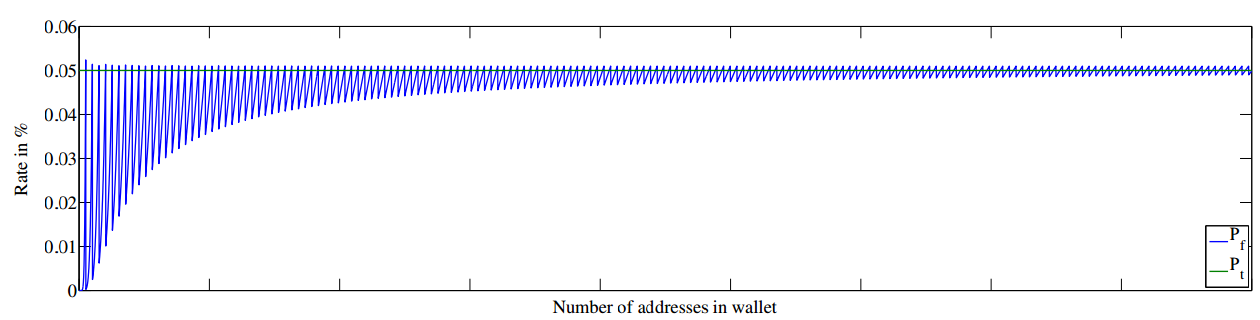
\includegraphics[width=\linewidth]{image/Pt_vs_Pf}
	\caption[مقادیر محاسبه شده برای $P_f$ و $P_t$ با توجه به تعداد آدرس‌های ($N$) قرار داده‌شده در فیلتر بلوم.]{%
		مقادیر محاسبه شده برای $P_f$ و $P_t$ با توجه به تعداد آدرس‌های ($N$) قرار داده‌شده در فیلتر بلوم. محور افقی این نمودار، نسبت $m$ فعلی فیلتر به $M$ انتخاب شده در زمان راه‌اندازی است.
		\cite{Gervais2014}}
	
	\label{fig:ptvspf}
\end{figure}


کوچک بودن 
$P_f(2N)$
نسبت به  
$P_t$
باعث می‌شود که امکان فاش شدن آدرس‌های اصلی فیلتر بلوم، در زمان راه‌اندازی فیلتر وقتی تعداد آدرس‌های آن کم باشد، بسیار بالاتر از حد انتظار باشد. به عنوان مثال، در یک فیلتر بلوم با $15$ آدرس و به تبع آن $30$ عنصر، مقدار $M=130$ خواهد بود. در نتیجه، با توجه به فرمول‌های 
\eqref{eq:n_of_bloom_filter}،
\eqref{eq:k_of_bloom_filter} و
\eqref{eq:Pf_of_bloom_filter_Mullin}
 برای نرخ خطای دوی هدف
$P_t=0.001$
 خواهیم داشت:
$n=1869$،
$k=10$ و
$P_f(30)=5.1\times10^{-9}$.

حال با توجه به فرمول \eqref{eq:P_h_estimation} احتمال آن‌که گره کامل متخاصم بتواند  یکی از آدرس‌های قرارگرفته در فیلتر بلوم را حدس بزند برابر 
$P_{h_{(1)}} = 0.99$
خواهد بود. به همین ترتیب گره کامل متخاصم می‌تواند با احتمال
$P_{h_{(15)}} = 0.8$
تمام آدرس‌های اصلی داخل فیلتر بلوم را حدس بزند. جدول \ref{table:P_h} از مقالهٔ \cite{Gervais2014} مقایسه‌ای بین تعداد آدرس‌های قرارگرفته در فیلتر بلوم در زمان راه‌اندازی و احتمال حدس زدن آدرس‌های آن توسط گره متخاصم را نشان داده است. توجه شود که مقادیر
$P_{h_{(.)}}$
نزولی اکید نیستند. از نظر شهودی نیز انتظار می‌رود که هرچه تعداد آدرس‌های یک فیلتر بلوم، در مقایسه با تمام آدرس‌های بیت‌کوین، افزایش پیدا کند، احتمال آن‌که آدرسی که در فیلتر بلوم منطبق است جزء آدرس‌های اصلی آن باشد بیش‌تر می‌شود. این ویژگی در مقادیر 
$P_{h_{(1)}}$
در جدول \ref{table:P_h} قابل مشاهده است. شکل \ref{fig:ph1} نموداری از احتمال حدس درست یک آدرس اصلی فیلتر بلوم با توجه به تعداد آدرس‌های آن در راه‌اندازی اولیه است. 
\begin{figure}
	\centering
	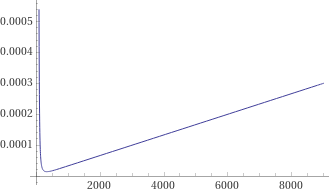
\includegraphics[width=0.7\linewidth]{image/P_h_1}
	\caption{%
		احتمال حدس درست یک آدرس اصلی فیلتر بلوم 
		($P_{h_{(1)}}$)
		با توجه به تعداد آدرس‌های آن ($N$) در راه‌اندازی اولیه.}
	\label{fig:ph1}
\end{figure}


\begin{table}
	
	\caption{%
		مقادیر 
		$P_{h_{(.)}}$
		با توجه به $N$
		($P_t=\%0.1$).
		\cite{Gervais2014}.
	}
	\label{table:P_h}
	\centering
	\begin{tabular}{|c|c|c|c|c|c|}
		\hline 
		\lr{$N$} & \lr{$1$} & \lr{$19$} & \lr{$49$}& \lr{$54$} & \lr{$8,999$}\\
		\hline
		\lr{$P_{h_{(1)}}$} & \lr{$1(\pm0)$} & \lr{$0.42(\pm0.03)$} & \lr{$0.0021(\pm0.00019)$} & \lr{$0.14(\pm0.0059)$} & \lr{$0.21(\pm0.00075)$}\\
		%----
		\lr{$P_{h_{([N/2])}}$} & \lr{$-$} & \lr{$0.000026$} & \lr{$0$} & \lr{$0$} & \lr{$0$}\\
		%----
		\lr{$P_{h_{([N])}}$} & \lr{$1$} & \lr{$0$} & \lr{$0$} & \lr{$0$} & \lr{$0$}\\
		\hline
 		
	\end{tabular}

\end{table}

	
در مقالهٔ \cite{Gervais2014} همچنین اثبات کرده است که اگر یک کاربر سبک دو فیلتر بلوم با اعداد تصادفی (\lr{nTweak}) متفاوت اما با اعضای دارای اشتراک تولید کند، احتمال آن‌که یک گره متخاصم $j$ عنصری که واقعا در فیلتر بلوم قرار دارند حدس بزند به صورت زیر محاسبه می‌شود:
\begin{equation}
\label{eq:P_h_multi_Bloom}
P_{h_{(j)}} \approx \prod_{k=0}^{j-1}\frac{N_1-k}{N_1+P_f(m_1)P_f(m_2)N_u-k}
\end{equation}

که
$P_{h_{(j)}}$
بدست آمده، به طور قابل ملاحظه‌ای، بیشتر از زمانی است که گره متخاصم تنها به یک فیلتر بلوم دسترسی داشته باشد \eqref{eq:P_h}. 

امکان جبران حدودی آسیب‌پذیری‌های گفته شده تا اینجا با اصلاح رفتار کاربر سبک وجود دارد. در قسمت \ref{change_behaviour} مروری بر کارهایی که کاربر سبکی که از بیت‌کوین‌جی استفاده می‌نماید می‌تواند انجام دهد تا بتواند تا حد ممکن آدرس‌هایش را از گره کاملی که از آن خدمات دریافت می‌کند حفظ نماید، انجام شده است. با این حال آسیب‌پذیری‌های دیگری برای این روش وجو دارد که نیاز به توجه بیشتر دارد.

آسیب‌پذیری دیگر آن‌ است که، به صورت کلی، در کاربرد‌های حفظ حریم خصوصی با استفاده از فیلتر بلوم، لازم است که به این مسئله توجه شود که اگر با قرار دادن آدرس $x$ در فیلتر بلوم، تعدادی بیت یک شود آیا هر کدام از این بیت‌ها از طریق قرار دادن یک یا چند عنصر پنهان‌سازی (خطای نوع دو) یک می‌شوند؟ به بیان دیگر اگر $b[i]$ فیلتر بلوم تنها توسط عنصر $x$ یک شود و نتوان آن بیت‌ را با قرار دادن عناصری غیر عضو ولی منطبق با فیلتر بلوم یک نمود، امکان حاشا کردن آنکه x در آدرس‌های مطلوب کاربر سبک قرار دارد، ممکن نخواهد بود. در نتیجه، اگر گره کامل متوجه شود که فقط به ازای یک آدرس $x$ خاص، خروجی توابع چکیده‌ساز به یک یا چند بیت مشخص نگاشت می‌شوند، می‌فهمد که حتما آدرس  $x$ جزء آدرس‌های اصلی قرار گرفته در فیلتر بلوم بوده است و گره سبک نمی‌تواند وجود آن آدرس را «حاشا» کند. مقاله \cite{Bianchi2012} ضمن اشاره به این آسیب‌پذیری، معیاری برای سنجش حریم خصوصی فیلتر بلوم با توجه به احتمال آنکه بیت‌های یک شده در فیلتر بلوم توسط عناصر غیر عضو پوشش داده شوند، ارائه کرده است که در بخش \ref{gamma-deniability} به آن پرداخته شده است.

یک مشکل اساسی دیگر روش استفاده از فیلتر بلوم \cite{Hearn2013}، بار پردازشی بسیار زیاد آن بر روی گره کامل ارائه دهندهٔ این سرویس است چرا که به ازای هر بلوک جدید باید تک‌تک عناصر مهم همهٔ تراکنش‌های بلوک را با تمامی فیلتر‌های بلومی که کاربران سبک با او به اشتراک گذاشته‌اند بررسی کند. هر بار بررسی وجود یک عنصر در یک فیلتر بلوم نیاز به چند مرتبه (حداکثر ۵۰ مرتبه) اجرای توابع چکیده‌ساز را دارد. از این رو گره کامل می‌تواند مورد 
%حملهٔ منع خدمت\RTLfootnote{\lr{Denial of Service Attack}} 
\gls{Denial of Service Attack}
قرار گیرد. کد منبع \cite{PeterTodd} یک کد پیاده‌سازی این حمله به زبان 
%پایتون\RTLfootnote{Python} 
\gls{Python}
است. با این حال تحلیل این آسیب‌پذیری نیاز به توجه بیشتری دارد.

آسیب‌پذیری دیگری که در ارتباط با پرسمان‌ گره سبک از گره کامل وجود دارد، تحلیل بسامد پرسمان یک آدرس  و مقایسهٔ پدیدار شدن آن در زنجیرهٔ بلوکی است. مسئلهٔ دیگر مقایسهٔ بازه‌های زمانی فعالیت یک گره سبک و آدرس‌هایی که در آن زمان در زنجیرهٔ بلوکی قرار گرفته و طبق فیلتر بلوم کاربر برای وی ارسال می‌شود، است. در این پایان‌نامه به صورت خاص بر روی این دو موضوع تمرکز شده است. 

در حال حاضر بسیاری از کاربران سبک بیت‌کوین هستند که جز سرمایه‌گذاری و نگه‌داری طولانی‌مدت بیت‌کوین فعالیت اقتصادی دیگری با آن انجام نمی‌دهند. این کاربران، خواه از کیف‌پول‌های سرد استفاده نمایند خواه نه، احتمال آن که همواره کیف پولشان در حال اجرا و هم‌گام سازی با شبکه باشد بسیار پایین است. در تلفن‌های همراه، به خاطر حفظ طول عمر باتری، در نتیجهٔ استفاده نشدن طولانی مدت از نرم‌افزار کیف پول، فعالیت‌‌های پس‌زمنیه‌‌ای کیف‌پول‌ها متوقف می‌شود.  

هرچند که متاسفانه تا کنون جمع‌آوری اطلاعاتی راجع به زمان‌های فعالیت گره‌های سبک و اتصال آن‌ها به گره‌های کامل انجام نشده است اما همچنان دور از ذهن نیست که فرض کنیم نرم‌افزار کیف پول کاربران کم فعالیت، اکثرا، فقط زمان‌هایی به شبکه متصل می‌شوند که بخواهند از قرارگیری تراکنشِ به تازگی منتشر شدهٔ خود در زنجیرهٔ بلوکی مطلع شوند یا اینکه بررسی کنند که تراکنشی که از طریق دیگری انتظار دریافتش را داشته باشند در زنجیرهٔ بلوکی ثبت شده باشد. 

به این ترتیب اگر فرض کنیم که گره سبک کم فعالیت $l_i$ در هر بار اتصال به یک گره کامل مشخص (مثلا $f_j$) در شبکهٔ بیت‌کوین  متصل شود، و تنها در زمان‌هایی که انتظار ثبت تراکنش مربوط به خودش را داشت، با شبکه همگام شود و در بازهٔ زمانی اطراف آن به پیام‌های \texttt{inv} از طرف گره کامل $f_j$ پاسخ‌ \texttt{getdata} را ارسال نماید، احتمال آن‌که تراکنش‌های منطبق شده با فیلتر بلوم کاربر که برایش ارسال می‌شوند، واقعا مربوط به کاربر سبک باشد، بسیار بیشتر خواهد بود. چرا که در آن بازه، از آن‌جایی که  تعداد تراکنش‌های به نسب کمتری در فیلتر بلوم آزموده می‌شوند،‌ تعداد تراکنش‌های حاصل از خطای نوع دو به نسبت بسیار کم خواهند بود. به این ترتیب گره $f_j$ با احتمال بیشتری می‌تواند مطمئن باشد که تراکنش‌هایی که به کاربری که به تازگی متصل شده است ارسال می‌شوند، مربوط به خودش است.  این آسیب‌پذیری در روش‌های بعدی که در فصل \ref{LitReview} به آن‌ها پرداخته خواهد شود نیز وجود دارد. هرچند در ابتدا فرض اتصال همیشگی به یک گره کامل یکسان ناشدنی به نظر بیاید، اما یک گره کامل متخاصم می‌تواند بدون نیاز به پرداخت هزینه‌ای، با اجرای 
%حملهٔ سیبیل\RTLfootnote{\lr{Sybil Attack}}
\gls{Sybil Attack}
هویت‌های جعلی زیادی در شبکه ایجاد نماید تا شانس ارتباطش با یک گره سبک را در به‌روزرسانی‌های او بالا ببرد. 

حملهٔ دیگری که می‌شود تعریف کرد که نسبت به حملهٔ قبلی شدنی‌تر باشد، آن است که گره کامل، سابقهٔ پرسمان‌های انجام شده از یک کیف پول به خصوص را ذخیره نماید. تشخیص این‌که پرسمان‌های صورت گرفته مربوط به یک کیف پول است می‌تواند از روی فیلتر‌های بلوم یکسانی که ارسال می‌شود تشخیص داده شود. همچنین اگر کاربر سبک فیلتر بلوم خود را عوض نماید اما از آدرس‌های یکسانی در فیلتر بلوم جدید هم استفاده کند،‌ گره کامل می‌تواند با مقایسهٔ آدرس‌های مشترک، به متعلق بودن هر دو فیلتر بلوم به یک کیف پول پی ببرد.

گره کامل متخاصم می‌تواند با تحلیل بسامدی که از یک کیف پول درخواست دریافت کرده است (با همان فرض قبلی که گره‌های سبک کم فعالیت ارتباطشان را به طور مداوم با گره کامل حفظ نمی‌کنند)، و مقایسهٔ آن با بسامد قرار گرفتن آدرس‌های منطبق شده بر فیلتر بلوم در زنجیرهٔ بلوکی، در مورد آدرس‌های اصلی قرار گفته شده در فیلتر بلوم اطلاعات کسب نماید. به عنوان مثال اگر یک کاربر سبک حدودا هر سه ماه یک‌بار به یک گره کامل متصل شود، گره کامل می‌تواند آدرس‌هایی که با فیلتر بلوم وی منطبق شده و روزانه در زنجیرهٔ بلوکی ظاهر شده‌اند را حذف نماید. از طرف دیگر کاربری که درخواست‌های زیادی انجام داده است، احتمال این‌که مالک آدرس‌های پر استفاده از فیلتر بلومش باشد بیشتر است. 

از طرف دیگر در روش فیلتر بلوم، گره کامل می‌تواند به بررسی روابط بین آدرس‌های منطبق شده با روش‌هایی مثل \cite{Meiklejohn2013} در یک فیلتر بلوم بپردازد. به این ترتیب می‌تواند احتمال بدهد که آدرس‌هایی که با فیلتر بلوم منطبق شده‌اند اما با آدرس‌های دیگر ارتباطی ندارند، جزء آدرس‌های پوششی فیلتر بلوم هستند\cite{Gervais2014}.  انتخاب تصادفی آدرس‌های خطای نوع دو می‌تواند شامل مشکلات دیگری نیز باشد، مثلا با توجه به \cite{Gervais2014} از آن‌جایی که فیلتر بلوم تازه در نیمهٔ دوم سال $2011$ معرفی شده است، اگر آدرسی که به عنوان خطای نوع دو با فیلتر بلوم منطبق شود مربوط به زمانی قبل‌تر از آن باشد ($2009$ تا $2011$)، گره کامل می‌تواند آن آدرس‌ها را با احتمال بالایی به عنوان خطای نوع دو فیلتر بلوم حساب نماید.

در این پایان‌نامه قصد داریم روشی را ارائه دهیم که کاربر سبک بتواند به صورت هوشمندانه آدرس‌های نامرتبط با خودش را به نحوی انتخاب نماید که بسامد استفاده از این آدرس‌ها برابر با نرخ استفاده از آدرس خودش باشد. همچنین در این روش کاربر سبک مجبور نخواهد بود که آدرس‌های مربوط به خودش را در یک ساختار دادهٔ واحدی مثل فیلتر بلوم قرار دهد که گره کامل بتواند با بررسی روابط بین آدرس‌های آن و آدرس‌های خطای نوع دو،‌ به آدرس‌های اصلی پی ببرد. بلکه چون گره سبک برای درخواست به روزرسانی هر آدرسش از یک سری مجموعه آدرس‌های پوششی نا مرتبط استفاده می‌کند و بقیهٔ آدرس‌های خودش را در آن‌ها قرار نمی‌دهد، گره کامل نمی‌تواند به ارتباط بین آدرس‌های مربوط به آن کاربر SPV پی ببرد. همچنین گره سبک می‌تواند به سادگی مجموعهٔ آدرس‌های خود را به روزرسانی کند، بدون آن‌که حریم خصوصیش از این بابت نقض شود.  


